% !TeX root = main.tex
% !TeX spellcheck = en-US
% !TeX encoding = utf8

\chapter{Theoretical Background} %Theoretical Foundations
\label{chap:background}
\glsresetall

\section{Traveling Salesman Problem}
\label{chap:tsp}

\subsection{A Brief History}

Having its basis in the mathematical theory around the Hamiltonian cycle in the 19th century, one of the first publications mentioning the term \textbf{\gls{tsp}} was done by \citefullauthor{robinson1949hamiltonian} in \citeyear{robinson1949hamiltonian} as part of an United States research company, a think tank called \enquote{RAND Corporation}, which offered its services to the U.S. armed forces \cite{schrijver2005history}. Besides \citeauthor{robinson1949hamiltonian}'s proposed solution, the scientific community at that time was very interested in the \gls{tsp}, applying all kinds of mathematical graph operations and often using branch-cutting algorithms to solve it \cite{lawler1985traveling}. The beauty of this problem lay in its simple, short description, which made it easy to understand, but also in its non-trivial and engaging solutions.

With advances in computer science also came more computationally applicable algorithms, such as the Kernighan–Lin heuristic \cite{lin1973effective}. At the same time, the \gls{tsp} was found to be NP-complete and therefore, NP-hard \cite{papadimitriou1976some} - a problem category that still remains a very interesting research topic in computer science. Through the work of \citet{dorigo1991ant} and the \enquote{ant system}, metaheuristics began to be a valid choice for solving the \gls{tsp} in the early 1990s. In parallel, with the emergence of the \textit{TSPLIB} benchmarking suite \cite{reinelt1991tsplib}, a wide adoption of said test instances began to compare and rank new algorithms and (meta-)heuristics.
Applications for the solutions are numerous, ranging from apparent routing of travel routes to frequency assignment \cite{punnen2007traveling}.

\subsection{Theory}
\label{chap:tsp-theory}
The problem description of the symmetric \gls{tsp}  can best be modeled by an undirected weighted graph $G = (V,E)$, with a set of $n$ vertices $V = \left\lbrace v_1, ... v_n\right\rbrace $ and a set of edges $E = \left\lbrace (v_i,v_j) | v_i,v_j \in V, i \neq j\right\rbrace $. Staying with the traveling salesperson analogy, the vertices are often being referred to as \enquote{cities}, while the edges between vertices represent the distance. This can be expressed by a distance function $d : V^2 \rightarrow \mathbb{R}_{0}^{+}$, which, in the case of the Euclidean \gls{tsp}, is just the Euclidean distance between two points in a two-dimensional space.  Each city can be visited only once, and since it is symmetric, it does not matter which direction the abstract salesperson travels. The problem is to find the shortest (i.e., smallest total distance) tour that visits each city exactly once, starting and ending in the same city. The solution is similar to a permutation of $V$, written as $\textbf{s} = (s_1,...,s_n) \in V^n$, that minimizes the sum over its distances, resulting in a solution quality function over $s$
\begin{equation}
	\label{eq:solution_quality}
	f(s) = L = \sum_{i=1}^{n} d(s_i,s_{i+1})
\end{equation}
with the city node $s_{i+1}$ coming after $s_i$ and $s_{n+1} = s_1$ to complete the full tour.
A more precise description of the problem is as follows: 


\begin{list}{}{}
	\item 	Given a weighted undirected graph, find the Hamilton cycle that minimizes the weight of all edges traversed.
\end{list}

In most cases, the graph is also complete, with every vertex connected to every other vertex. Especially for computational tasks, it is often easier to view the \gls{tsp} description as a distance matrix defined as follows:
\begin{equation} 
	\label{eq:dist_matrix}
	\textbf{D} = \left\lbrace d(v_i,v_j) \right\rbrace_{nxn}
\end{equation}
An example of a simple \gls{tsp} instance is shown in Fig. \ref{fig:ExampleTSP}; its distance matrix would then be:
$$
\textbf{D} =
 \begin{bmatrix}
	0 & 7 &7 & 10\\
	7 & 0 & 10 & 7\\
	7 & 10 & 0 & 7\\
	10 & 7 & 7 & 0\\
\end{bmatrix}
. $$
  \begin{figure}
  	\centering
 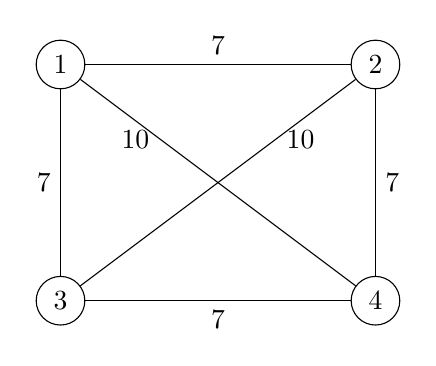
\begin{tikzpicture}
	\node[circle,draw] (1) at (4,8)  {$1$};
	\node[circle,draw] (2) at (8,8)  {$2$};
	\node[circle,draw] (4) at (4,5)  {$3$};
	\node[circle,draw] (3) at (8,5)  {$4$};
	\draw[-] (1) -- node[above] {7} (2);
	\draw[-] (2) -- node[right] {7} (3);
	\draw[-] (3) -- node[below] {7} (4);
	\draw[-] (4) -- node[left] {7} (1);
	\draw[-] (1) -- node[pos=.2,below] {$10$} (3);
	\draw[-] (2) -- node[pos=.2,below] {$10$} (4);
\end{tikzpicture}
    \caption{Example of a symmetric \gls{tsp} instance with $n=4$ cities}
    \label{fig:ExampleTSP}
\end{figure}


There are several modifications of this standard problem. The asymmetric \gls{tsp} (ATSP) has the added complication that the weights between the vertices are different depending on the direction the edge is being traversed, such that $d(v_i, v_j) \neq d(v_j,v_i)$, which increases the complexity and optimization potential for these instances \cite{johnson2007experimental}.
The \gls{dtsp} incorporates certain dynamic aspects, such as changing edge weights or inserting, deleting, or swapping city nodes, into the problem domain. It is different in the sense that it has neither a specific problem description nor universally valid solutions, since this all depends strongly on the implementation. The basis is often a traditional symmetric \gls{tsp} instance with some form of the above mentioned dynamic changes applied deterministically or randomly over time $t$. Therefore, the distance matrix in Eq. \eqref{eq:dist_matrix} becomes time-dependent $\textbf{D}(t)$. Searching for solutions to an ever-changing problem increases the importance of a good anytime behavior of the algorithm or metaheuristic, with the ultimate goal of finding the best possible solution at any given moment, so Eq. \eqref{eq:solution_quality} also becomes time-dependent $f(s,t)$. 


\section{Metaheuristics}
\label{chap:meta}

Solving a hard optimization problem with an exact (deterministic) method may yield the optimal solution to the problem, but often at the cost of high computational intensity. And although it is often mathematically proven that an optimal solution can be reached in reasonable time, this time can be considerably long. A metaheuristic generally does not deal with exact solutions, but rather tries to find the \textit{best} solution in a given, often small enough, time frame. 
Furthermore, a heuristic algorithm requires specific knowledge about the problem it is solving, whereas metaheuristics are generally adaptable to a larger space of optimization problems and do not expect the problem's formulation to be of such strict a format \cite{sorensen2013metaheuristics}. 
Algorithms of this type often include strategies to balance the exploratory and exploitative search behavior. The exploration aspect tries to find promising areas within the (complex) search space containing good solutions, while the exploitation feature tries to specify the exact solution in those promising areas, also to gain experience. This principle is one of the main distinctions between different metaheuristics and their configuration \cite{boussaid2013survey}.

From the Greek prefix \textit{meta}, roughly translated as \textit{high-level}, a metaheuristic can be understood as a \enquote{high-level, problem-independent algorithmic framework} \cite{sorensen2013metaheuristics} that is capable of employing strategies to generate processes of heuristic nature that are able to escape local optima as well as robustly search a solution space. The latter is especially true for population-based metaheuristics \cite{gendreau2010handbook}. 
The framework perspective is particularly important, because the general descriptions of metaheuristics often include certain operations that are combined to achieve the above mentioned functionality. Therefore, a metaheuristic can be more of a concept for designing an algorithm, rather than a strict specification of an implementation. This understanding has also given rise to so-called \enquote{hybrid metaheuristics}, which mix and match ideas from several frameworks into one algorithm \cite{sorensen2018history}.

Giving a definitive taxonomy of metaheuristics is impractical because there are many characteristics that can distinguish them. 
One of the more common ones are based on...
\begin{itemize}
	\item ...solution creation quantity: Single-Solution Based vs. Population-Based
	\item ...solution creation process: Deterministic vs. Probabilistic/Stochastic
	\item ...how solutions are manipulated:\\ Local Search vs. Constructive vs. Population-Based \cite{sorensen2013metaheuristics}
	\item ...which analogy they belong to:\\ Bio-Inspired vs. Physics-Based vs. Evolutionary  vs. Swarm-Based
\end{itemize}

Although all of these classifications are justified, none of them will be used alone, as it would serve no purpose to limit the discussion to one category. When necessary, algorithms are placed within these taxonomies, to explain their purpose respectively.

\subsection{Overview}

The first classification mentioned (Single-Solution Based vs. Population-Based) is used to provide a brief overview of the field because it provides an intuitive separation. 

\subsubsection{Single-Solution Based Metaheuristics}

\Glspl{smeta} improve on a single, initial solution and describe a trajectory as it moved through the search space. Hence, they are often referred to as \textit{trajectory methods}. The dynamics applied to each new iteration of solutions depend heavily on the specific strategy. However, they can generally be described by a generation procedure, where new candidate solutions are generated from the current one, and a replacement procedure, where one of the new solutions is selected based on some criteria \cite{talbi2009metaheuristics}. A very important aspect in finding new solutions during the first phase is the neighborhood structure. It represents the accepted area in the search space around the current solution, and its definition is usually very much dependent on the problem it is associated with. A larger neighborhood may increase the chance of \enquote{jumping} over local optima, but at the cost of more computation.
\begin{algorithm}
	\caption{Basic Local Search}
	\label{alg:basiclocalsearch}
	
	\begin{algorithmic}
		
		\State $s \gets $ \Call{GenerateInitialSolution}{ }
		\Repeat
		\State $ s'  \gets $ \Call{Generate}{$N(s)$}
		\If{\Call{Select}{$s'$}} 
		\State $ s \gets s' \in N(s)$
		\EndIf
		\Until{termination criterion met}
	\end{algorithmic}
\end{algorithm}

 \Cref{alg:basiclocalsearch} shows a high-level description for one of the first and simplest \glspl{smeta}, the Basic Local Search. The functions (generate, select) and the neighborhood $N$ vary depending on the implementation. For example, the generation of new solutions can be of deterministic or stochastic nature, while the selection of a candidate may be based on the best improvement found in the entire neighborhood or based on the first improvement that occurs \cite{talbi2009metaheuristics}. The greatest issue with Basic Local Search is convergence to local optima, and most other implementations of a \gls{smeta} extend this algorithm to counteract this flaw in some way \cite{blum2003metaheuristics}. 
 
 One of these is \gls{sa}, which is based on the physical process of annealing. When a metal is heated above its recrystallization temperature and is then cooled in a controlled manner, its atoms are able to reside into a lower energy state, altering the metal's properties. This analogy is used to simulate a temperature that controls the magnitude of change between possible solutions. A higher temperature allows for worse solutions than the current one, which, hopefully, allows for \enquote{climbing} out of local optima. As the algorithm progresses, the virtual temperature cools down, decreasing the chances for such uphill moves and \gls{sa} eventually converges to a simple local search algorithm \cite{blum2003metaheuristics}.
 
\Gls{ts}, on the other hand, uses a list (\textit{memory}) to explicitly utilize the search history to its benefit. In its simplest form, \gls{ts} uses a \textit{short-term memory} to remember the most recent solutions, limiting the neighborhood to solutions not present in the list. Thus, larger lists force the algorithm to explore larger search spaces.
Other, more recent \glspl{smeta} algorithms include \textit{Iterated Local Search} (ILS), \textit{Greedy Randomized Adaptive Search Procedure} (GRASP), and \textit{Variable Neighborhood Search} (VNS) \cite{talbi2009metaheuristics}.

\subsubsection{Population-Based Metaheuristics}

The common aspect with \glspl{pmeta} is that they maintain an entire set (\textit{population}) of solutions. This presence of multiple solutions results in an intrinsic drift toward a more exploratory algorithmic behavior \cite{blum2003metaheuristics}. 
Although they do not share the same algorithmic background as many \glspl{smeta}, they have similarities when it comes to improving their populations. Starting with a population generation phase, new solution sets are iteratively created by each member of the population (generation phase) and then incorporated into the current population or even replaced by it (replacement phase) until a stopping criterion is satisfied. The last two of these three phases may even use some sort of solution history to build their functions, or operate completely memoryless. The choice of initial population also plays a significant role in the diversification behavior and computational cost of the algorithm  \cite{talbi2009metaheuristics}. 

Algorithms with analogies to swarm intelligence, often found in animals in nature, are an example of \glspl{pmeta}. These types of algorithms typically work with agents that are individually not complex and use simple operations to build a solution. However, they exchange information and move cooperatively through the problem space. Two examples of swarm-intelligence based algorithms are described in the next two subsections. Other popular examples of \glspl{pmeta} are \glspl{ea}, which refer to biologically inspired operations such as mutation and recombination to manipulate their population, or Scatter Search (SS).


\subsection{Ant Colony Optimization}
\label{chap:aco}

The \gls{aco} in its original form (\enquote{Ant System} as proposed by \citet{dorigo1996ant}) is a multi-agent metaheuristic inspired by the foraging behavior of real ants.
 Through ethological studies it was found that ants, although nearly blind \footnote{The visual ability of ants varies according to species and function in the colony. The studied Argentine ant (Linepithema humile) has very poor vision \cite{talbi2009metaheuristics}.}, are able to find very short paths between a food source and their nest \cite{goss1989self}. This is achieved by a chemical substance produced by the ant, called pheromone, which is deposited along the path it has traveled. Without any pheromone information to guide them, ants travel mostly at random. However, when an ant encounters a pheromone trail, there is a high probability of following it, thus reinforcing this path with its own pheromone. This autocatalytic (positive feedback) behavior is counteracted by the volatility of the pheromone, which dissipates over time, weakening path reinforcement \cite{dorigo1996ant}. This results in the shorter paths accumulating higher amounts of pheromone, as shown in \cref{fig:aco-obstacle}. This example also shows the response to a dynamic change in the path, which is an obstacle placed directly on the shortest route. Although the left path is initially as likely as the right path, the reinforcement on the shorter right path is greater, causing the ants to adapt to the obstacle \cite{talbi2009metaheuristics}. However, the removal of the obstacle in this example would not lead to a return to the old path, because of the already reinforced pheromone trail \cite{dorigo2004ant}.

\begin{figure}[h]
	\centering
	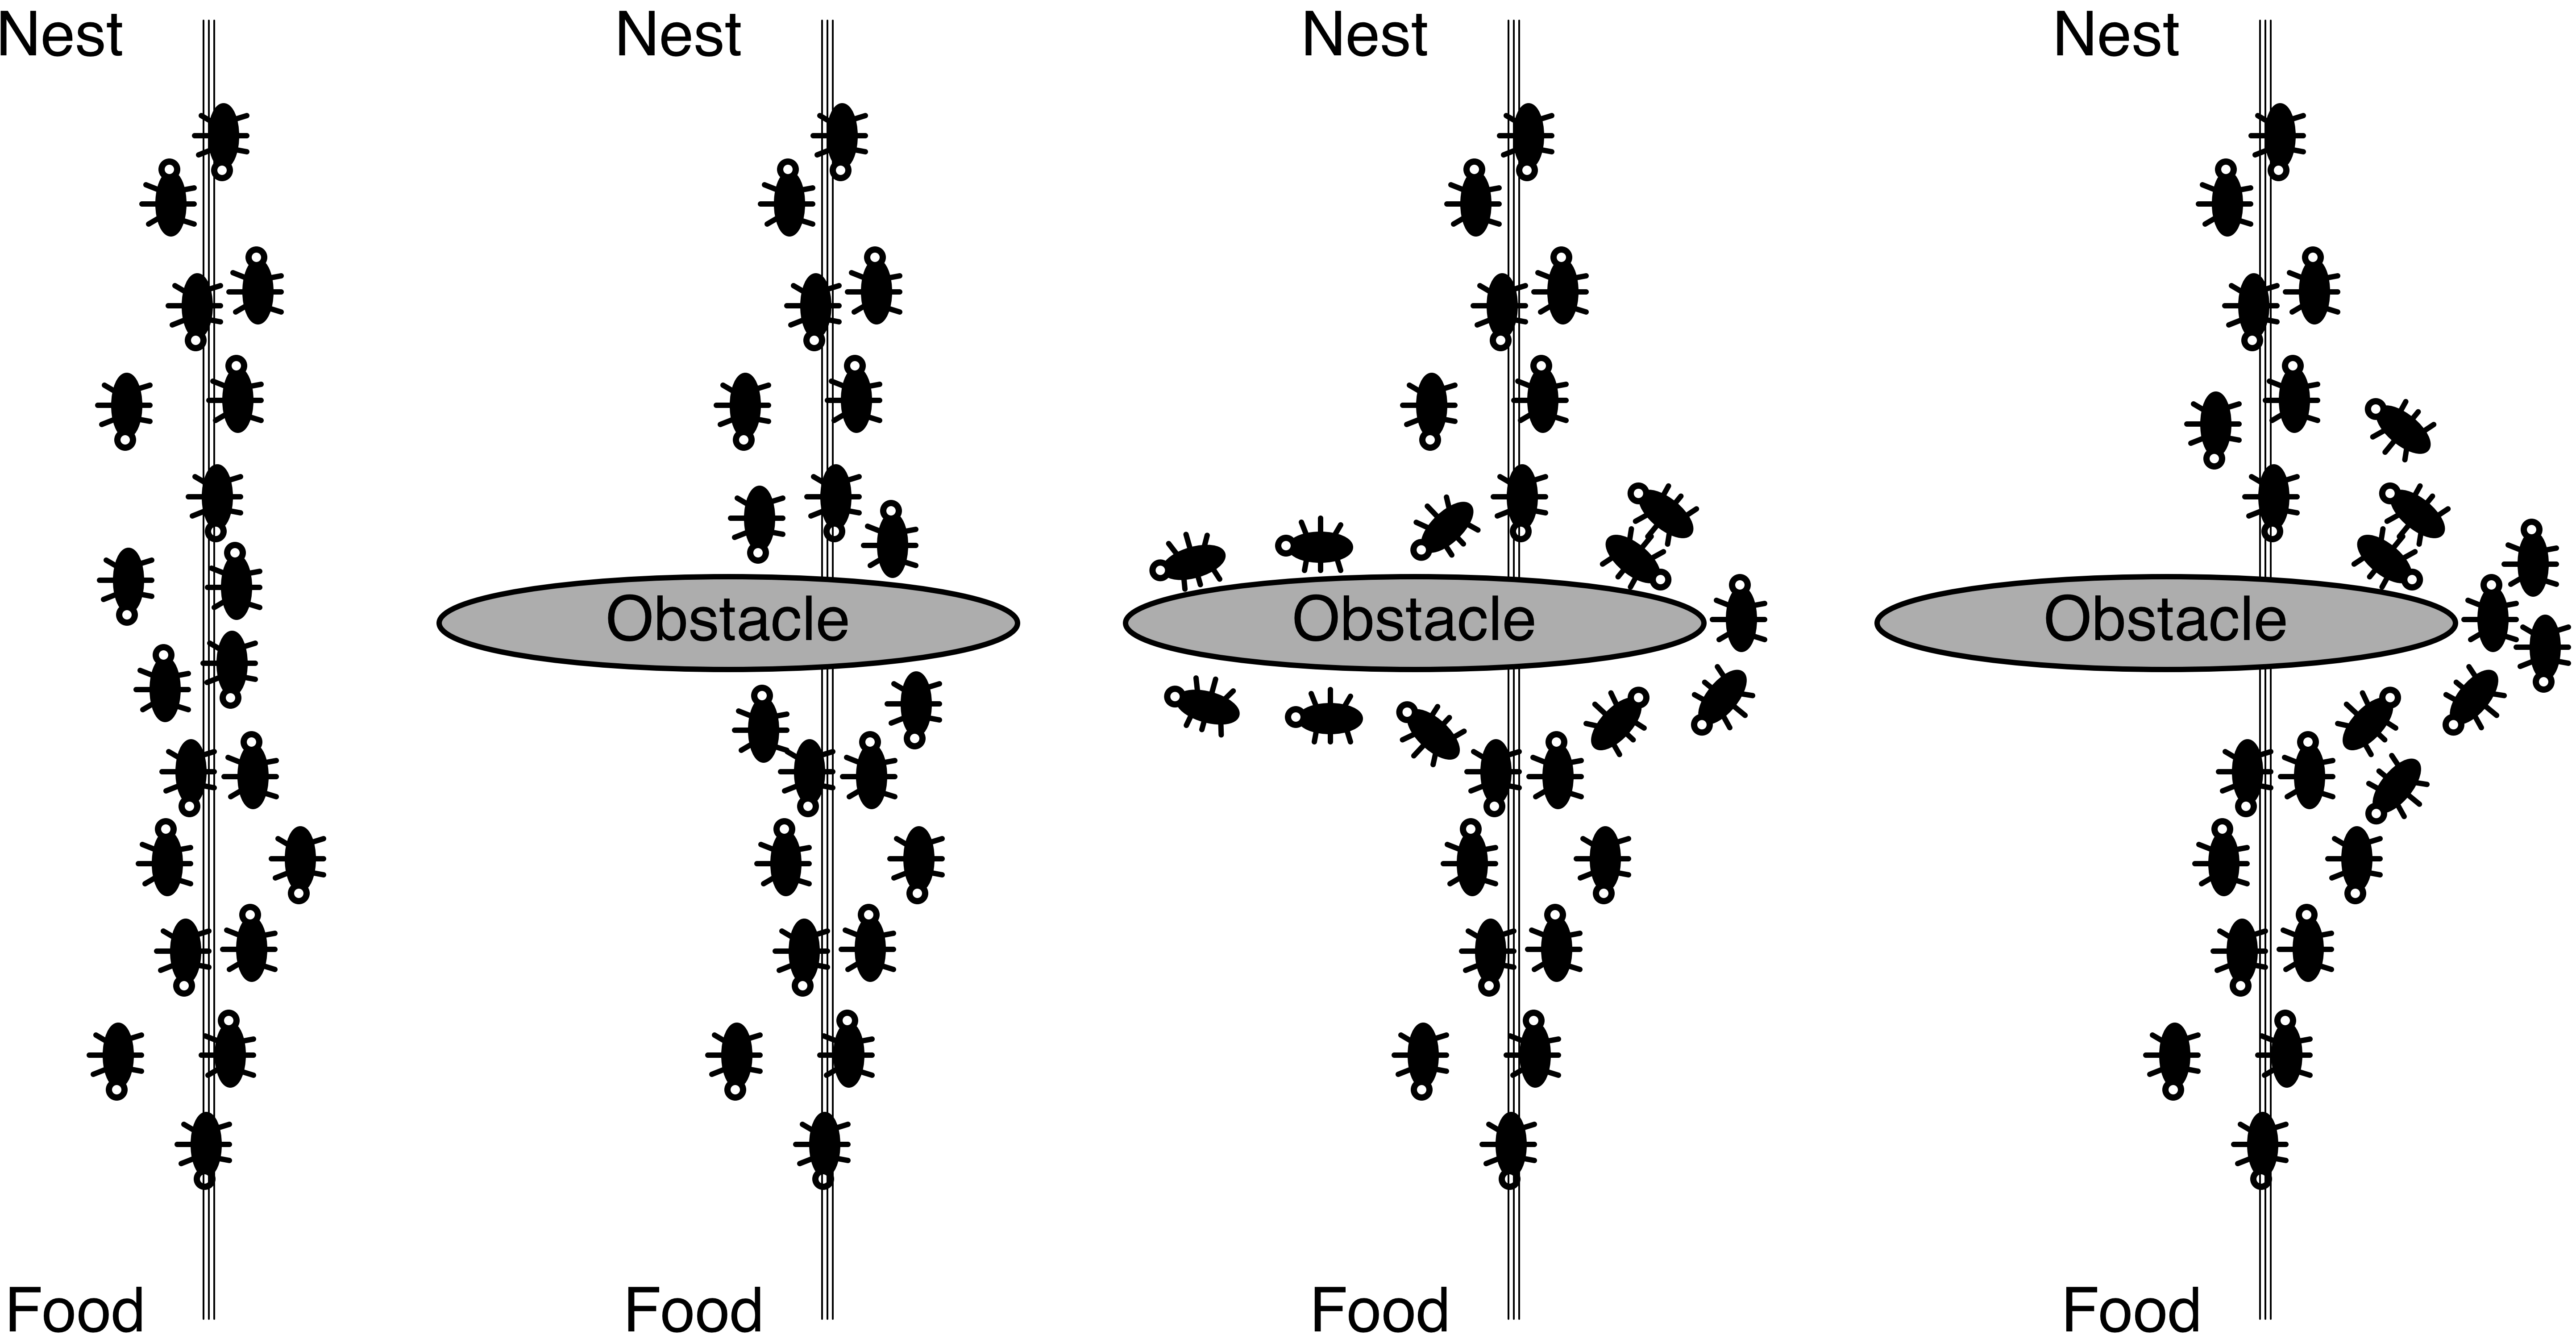
\includegraphics[width=0.85\textwidth]{aco-obstacle.png}
	\caption[The process of ants following a pheromone trail]{The process of ants following a pheromone trail between a food source and their nest affected by an obstacle. Modified from \citet{talbi2009metaheuristics}.}
	\label{fig:aco-obstacle}
\end{figure}

The artificial ants in \gls{aco} are inspired by this behavior and iteratively build a solution by probabilistically choosing the next part based on heuristic, problem-specific information, and, analogous to the real ants, artificial pheromone information. The use of multiple agents also gives the algorithm more robustness and diversification in solving a problem \cite{dorigo2019ant}.

\begin{algorithm}
	\caption{Ant Colony Optimization}
	\label{alg:aco}
	
	\begin{algorithmic}
		\State Initialize pheromone information
		\Repeat
		\For{each ant}
		\State \Call{ConstructSolution}{}
		\EndFor
		\Procedure{UpdatePheromones}{}
		\State \Call{Evaporation}{}
		\State \Call{Reinforcement}{}
		\EndProcedure
		\Until{termination criterion met}
	\end{algorithmic}
\end{algorithm}

The algorithmic implementation is quite straightforward. And since its original use was often adapted for the \gls{tsp}, and this thesis solves that problem as well, the following description is slightly modified to fit it.
\Cref{alg:aco} shows the basic template of the \gls{aco}. First, the pheromone information is initialized uniformly, so that each path is initially equally likely to be chosen. With a total of $n$ cities to visit, the resulting matrix is of dimension $n \times n$, where each entry $\tau_{ij}$ represents the amount of pheromone being present at the edge $(i,j)$.
For every complete cycle, each of $m$ ants probabilistically creates a solution with this pheromone information $\tau_{ij}$ and heuristic information $\eta_{ij}$. Starting from a randomly selected city $i$, the probability to visit the next possible city $j$ from a set $S$ of not yet visited cities is given by 
\begin{equation}
		\label{eq:aco_prob}
		p_{ij} = \frac{\tau_{ij}^\alpha \cdot \eta_{ij}^\beta}{\sum_{h \in S} \tau_{ih}^\alpha \cdot \eta_{ih}^\beta}
\end{equation}
where $\eta_{ij}$ holds the problem specific heuristic value, which is the inverse distance $\eta_{ij} = \frac{1}{d_{ij}}$ between cities $i$ and $j$ in case of the \gls{tsp}. The constants $\alpha, \beta \geq 0$ control the influence of either the stochastic pheromone or the heuristic value. The denominator normalizes the fraction into a probability $0 \leq p_{ij} \leq 1$, with the set of all probabilities from the unvisited cities $S$ effectively creating a probability distribution \cite{talbi2009metaheuristics}.

The pheromone information is then updated based on the generated solutions. First, each pheromone entry is subject to evaporation controlled by a constant value $\rho \in (0,1]$ and defined by the following equation:
\begin{equation}
	\label{eq:aco_evap}
	\forall i,j \in [1,n]: \tau_{ij} \leftarrow (1-\rho) \cdot \tau_{ij}
\end{equation}
In the following reinforcement phase, different strategies can be applied to select how the solutions chosen by the ants influence the pheromone matrix. There are also versions of the \gls{aco} where this procedure is called after each step of the solution construction, or at least after a single ant, but not necessarily after each ant has finished constructing its solution. More common, however, are offline strategies that are called after each ant has finished. One of the simpler implementations in this category is the \enquote{elitist pheromone update}, where the updates of the pheromone matrix are strongly influenced by the global best solution. Another approach is the \enquote{quality-based pheromone update} or \enquote{ant-cycle} \cite{dorigo1996ant}, where each ant $k = 1,2,...,m$ updates the pheromone matrix relative to the length of the solution $L_k$ they found in that iteration, which is further controllable by a parameter $Q \geq 1$. The following two equations define this strategy:
\begin{equation}
	\tau_{ij} \leftarrow \tau_{ij} + \sum_{k=1}^{m} \Delta\tau_{ij}^k 
\end{equation}
\begin{equation}
	\Delta\tau_{ij}^k = \begin{cases}
		\frac{Q}{L_k}, &\text{if edge } (i,j) \text{ is in $k$-th ant tour,} \\
		0, &\text{otherwise}
	\end{cases}
\end{equation}

This loop is repeated until a termination criterion is met. This can be a fixed number of iterations $\text{NC}_{\text{MAX}}$ or until the solution quality stagnates for a certain number of iterations. With the pheromone update implemented as an \enquote{ant-cycle} the time complexity of this algorithm is $O(\text{NC}\cdot n^2 \cdot m)$ \cite{dorigo1996ant}. Based on this algorithm, a large number of variants have been created. One of them is a population-based approach, which is discussed in the following.

\subsubsection{Population-Based Ant Colony Optimization}
The \gls{paco} was first proposed by \citet{guntsch2002population} as a simplification of the \gls{aco}, effectively reducing the operations required to update the pheromone information by quantifying and limiting the values added to the matrix. Their motivation was to speed up the process and reduce the influence of older solutions in order to apply the \gls{paco} to the \gls{dtsp}. 
Instead of storing all updates to the pheromone matrix, the approach keeps track of the solutions that have updated the solution in a queue, called the \textit{population}. Therefore, every solution in this queue is actually present in the matrix and vice versa. To limit the influence of old solutions, the population size is set to a value $k$. When the queue is full after $k$ iterations, several actions are possible in iteration $k+1$, with the most obvious being to implement a FIFO (first in, first out) behavior, discarding the oldest solution. This also eliminates the need for evaporation. The rest of the algorithm is analogous to the \gls{aco} presented earlier. The matrix is initialized with a constant amount $\tau_{\text{init}}$. The pheromone update is done by the ant with the iteration best solution. With a weight $w_e \in [0,1]$ controlling the amount of pheromone deposited and a maximum set to $\tau_{\text{max}}$, the amount of pheromone added is defined by $(1-w_e) \cdot (\tau_{\text{max}} - \tau_{\text{init}})/k$.
This reduces the number of pheromone updates per generation, for a \gls{tsp} instance of $n$ cities, from $n^2$ operations to at most $2n$ operations \cite{guntsch2002population}.

\begin{figure}
	\hfill
	\begin{subfigure}{.3\textwidth}
		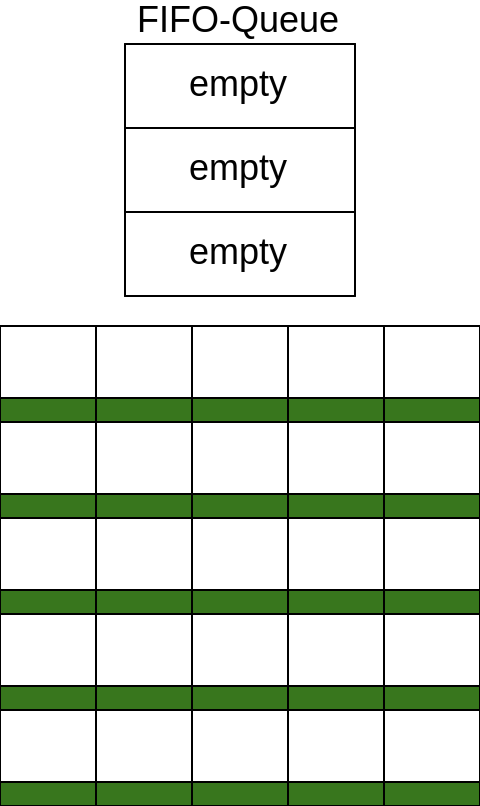
\includegraphics[width=\textwidth]{paco-1.svg}
		\caption{Matrix at $i=0$}
		\label{fig:paco1}
	\end{subfigure}
	\hfill
	\begin{subfigure}{.3\textwidth}
		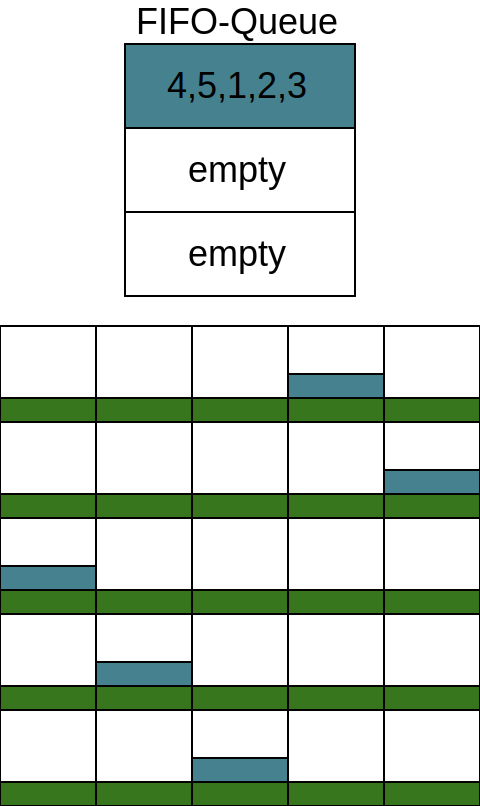
\includegraphics[width=\textwidth]{paco-2.svg}
		\caption{Matrix at $i=1$}
		\label{fig:paco2}
	\end{subfigure}
	\hfill
	\begin{subfigure}{.3\textwidth}
		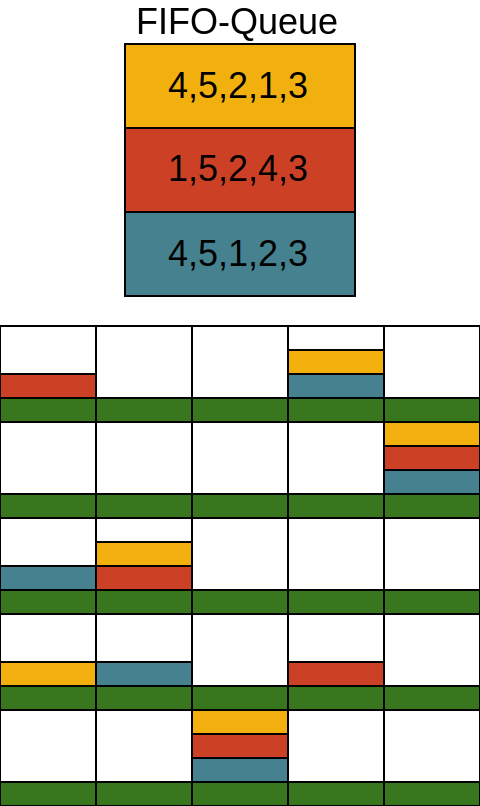
\includegraphics[width=\textwidth]{paco-3.svg}
		\caption{Matrix at $i=3$}
		\label{fig:paco3}
	\end{subfigure}
	\caption[Example of a \gls{paco} matrix being updated over multiple iterations]{Example of a \gls{paco} matrix being updated over multiple iterations for a solution population size of $k=3$. The rows represent the location of the solution ranging from $1$ to $n$, while the columns depict the option chosen (e.g., a city node for the \gls{tsp}).}
	\label{fig:paco}
\end{figure}

\Cref{fig:paco} shows an example of a pheromone matrix with a solution population of $k=3$ being updated over the course of three iterations for a problem of size $n$. In \cref{fig:paco1}, the population is empty and the matrix is initialized with $\tau_{\text{init}}$, visualized by the green bars. The best solution of the first iteration has the city referenced at position 4 as it's start, continuing with position 5, and so on. This update is visualized by blue colored bars. Eventually, after two more iterations (\cref{fig:paco3}), the population queue is full. In a next iteration, the solution visualized in blue would leave the matrix and a new one would be placed at the top of the queue.

\subsection{Particle Swarm Optimization}

The \gls{pso} method was introduced by \citet{kennedy1995particle} as a \enquote{concept for optimization of nonlinear functions} by simulating swarms of birds or fish in their search for food. The individuals, referred to as \textit{particles}, iteratively explore a given problem space of dimension $d$. Therefore, each of the $N$ particles in a swarm represents a candidate solution to the problem, evaluated by an objective fitness function $f: \mathbb{R}^d \to \mathbb{R}$. Furthermore, each particle $i$ is defined by three vectors and two values:
\begin{itemize}
	\item the current position $\vec{x_i} \in \mathbb{R}^d$ 
	\item the current velocity $\vec{v_i} \in \mathbb{R}^d$ 
	\item the best solution found so far $\vec{p_i} \in \mathbb{R}^d$
	\item the fitness values $f(\vec{x_i})$ and $f(\vec{p_i})$
\end{itemize}

To let the particles influence each other, a neighborhood rule must be defined. The most straightforward way is the global best method (\textbf{gbest}), where all particles influence each other without restrictions. Another, potentially more complex, strategy for letting the particles exchange information is the local best method (\textbf{lbest}). In this method, particles interact based on a given topology, such as a ring, where only direct neighbors exchange information. Thus, regardless of the strategy chosen, each neighborhood $k$ has a leader with the best solution $\vec{g_k}$ \cite{talbi2009metaheuristics}. Putting both aspects together, the particles update their velocity based on personal success (\textit{cognitive aspect}) and neighborhood success (\textit{social aspect}) \cite{janson2003hierarchical}. 

\begin{algorithm}
	\caption{Particle Swarm Optimization}
	\label{alg:pso}
	\begin{algorithmic}
		\State Initialize swarm
		\Repeat
		\ForAll{particles $i \in [1, N]$}
		\State \Call{UpdateVelocities}{}
		\State \Call{UpdatePosition}{}
		\If{$f(\vec{x_i}) < f(\vec{p_i})$} {$\vec{p_i} = \vec{x_i}$}
		\If{$f(\vec{x_i}) < f(\vec{g_k})$} {$\vec{g_k} = \vec{x_i}$}\EndIf \EndIf
		\EndFor
		\Until{termination criterion met}
	\end{algorithmic}
\end{algorithm}

\Cref{alg:pso} shows a high-level description of the \gls{pso} procedures. Typically, the swarm is randomly initialized, with each particle assigned a velocity and a position in the search space. The resulting solutions are set as $\vec{p_i}$ and, for each particle's neighborhood $k$, the leader solution $\vec{g_k}$ is determined. After the initialization, each particle $i$ updates its velocity $\vec{v_i}$ per iteration $t$ according to the following equation:
\begin{equation}
	\vec{v_i}(t+1) = w \cdot \vec{v_i}(t) + c_1 \cdot r_1 \cdot (\vec{p_i} - \vec{x_i}(t)) + c_2 \cdot r_2 \cdot (\vec{g_k} - \vec{x_i}(t))
\end{equation}

with an inertia weight $w > 0$ that controls the influence of particle velocity. The parameters $c_1, c_2 > 0$ define the influence of the personal best $\vec{p_i}$ and the neighborhood best solution $\vec{g_k}$, respectively and are additionally subject to a random factor due to values $r_1, r_2$ drawn from a uniform distribution of $[0,1]$. Afterwards, the particle's position is updated: 
\begin{equation}
	\vec{x_i}(t+1) = \vec{x_i}(t) + \vec{v_i}(t+1)
\end{equation}  
Lastly, the best solutions are potentially updated if they are better than the current ones. To ensure convergence of the swarm, many implementations also limit the velocity to a certain value or reduce the inertia weight over time.
This whole process is visualized in \cref{fig:pso-vector}, which shows a particle $i$ being updated according to all three possible influences. 

  \begin{figure}
	\centering
	\begin{tikzpicture}[thick,>={Triangle[angle=30:4pt 4]}]
		\coordinate[label={[xshift=-10]left:{$x_i(t)$}}] (O) at (0,0);
		\coordinate[label=0:{$p_i$}] (A) at (1,2);
		\coordinate[label=0:{$g_k$}] (B) at (5,1);
		\coordinate (C) at (2,-2);
		\coordinate (C2) at (1.9,-2.1);
		\coordinate[label={[xshift=+10pt]right:{$x_i(t+1)$}}] (S) at ($0.5*(A)+0.3*(B)+0.8*(C)$);
		\coordinate (S1) at ($(O)+0.8*(C)$);
		\coordinate (S2) at ($(S1)+0.5*(A)$);
		\coordinate (S3) at ($(S2)+0.3*(B)$);
		
		\node[fill=gray,circle,left,radius=5pt] at (O) {};
		\node[fill=gray,circle,right,radius=5pt] at (S) {};
		
		\draw[->] (O) -- (A) node[midway,auto] {$p_i - x_i(t)$} ;
		\draw[->] (O) -- (B) node[midway,above] {$g_k - x_i(t)$} ;
		\draw[->] (O)+(-0.1,-0.1) -- (C2) node[midway,below left] {$v_i(t)$} ;
		\draw[->, dashed] (O) -- (S1) ;
		\draw[->, dashed] (S1) -- (S2) ;
		\draw[->, dashed] (S2) -- (S) ;
	\end{tikzpicture}
	\caption[The vector summation of a \gls{pso} particle]{The vector summation of a \gls{pso} particle $i$ during velocity and position update.}
	\label{fig:pso-vector}
\end{figure}

Research has been performed to understand how the algorithm behaves and how to vary the algorithm. In particular, the choice of neighborhood topology has a significant impact on performance. The \textbf{gbest} method seems to perform better on unimodal problems, where there is one clear function optimum, while the \textbf{lbest} method gives better performance on multimodal problems with many optimal function values \cite{janson2003hierarchical}. 

\label{chap:hpso}
One such variant is the \gls{hpso} proposed by \citet{janson2003hierarchical}, which uses a hierarchical tree topology (indicating solution quality) to define a neighborhood. The resulting (almost) regular tree has a total number of $m$ nodes over a height $h$, where each parent node has at most $d$ children. The particles are represented by the nodes of the tree, and, therefore, the neighborhood of each particle $i$ is defined only by its direct parent $j$ in this hierarchy, so $\vec{g_i} = \vec{p_j}$. 
The updating of velocity and position remain the same as in the standard approach, but the comparison and eventual update of the neighborhood best solution $\vec{g_k}$ can be seen as a tree restructuring process. If a child node $i$ happens to find a better solution than its parent node $j$, so $f(\vec{p_i}) < f(\vec{p_j})$, they swap their position in the hierarchy. This process is performed top-down, breadth-first, resulting in worse solutions may moving down several levels in an iteration, but good solutions moving up at most one level. The global best solution can then be found at the root position after a maximum of $h$ iterations.

Another variant is called \gls{sso}, which is a discrete version of the \gls{pso}, capable of solving combinatorial problems such as the \textit{MMRAP} (multi-level, multi-state redundancy allocation problem), as proposed by \citet{yeh2009two}. The solution of the particle is no longer represented by the position and the velocity in the multidimensional problem space, but is instead encoded as a finite-length string and an additional fitness value. The update mechanism has also been simplified by probabilistically selecting the next position string based on a random number that may lie in multiple tunable intervals \cite{yeh2012simplified}. These intervals are the probabilities for the personal best solution $p_{\text{pbest}}$, the personal previous solution $p_{\text{pprev}} $ and the global best solution $p_{\text{gbest}}$. The resulting solution vector $\mathbf{s}^t_j$ for particle $j$ at iteration $t$ is therefore built according to
\begin{equation}
	\label{eq:sso_rule}
	s_{ij}^{t+1} = \begin{cases}
		s^t_{ij} & \text{ with propability } p_{\text{pprev}}, \\
		p^t_{ij} & \text{ with propability } p_{\text{pbest}}, \\
		g^t_{i} &\text{ with propability } p_{\text{gbest}}, \\
		v & \text{ with propability } p_{r}
	\end{cases}
\end{equation}
with $s_{ij}$ being the $i$-th solution component of particle $j$ and $v \in V$ being a value from a set of all feasible values chosen with probability $p_r$ \cite{lin2015simple}. 


\subsection{SPPBO Framework and H-SPPBO Algorithm}

\subsubsection{Simple Probabilistic Population-Based Optimization}

The \gls{sppbo} is a metaheuristic scheme that combines generalized aspects of population based approaches, such as \gls{pso} and \gls{sso}, and strategies that effectively generate probability distributions, such as \gls{aco} and \gls{paco}. As discussed by \citet{lin2015simple}, the framework can be used to classify and virtually recreate many of these metaheuristics for solving discrete combinatorial problems by using two simple operations: 
\begin{itemize}
	\item \textit{SELECT+COPY}: Selecting a solution from the population and copying (parts of) this solution when certain conditions apply.
	\item \textit{RANDOM}: Random selection of a value from the set of possible values.
\end{itemize}
These operations can be used to create multiple variants of an \gls{sppbo} algorithm, as well as de facto implementations of \gls{paco} and \gls{sso}. However, they all share the same schematic foundation. First, a distinction must be made between populations and \glspl{sce}. Reminiscent of an ant (\gls{aco}) or a particle (\gls{paco}),  a set of \glspl{sce} $\mathcal{A}$ create the solutions by applying probabilistic rules $\text{Prob}_V$ and, optionally, some form of heuristic information $\eta$. These solutions may then enter a set of populations $\mathcal{P}$ (cmp. \gls{paco}). $V$ denotes the set of possible values $v_i \in V$ that may appear in a solution vector $\textbf{s} \in V^n$ of length $n$. 
The high-level structure of these \gls{sppbo} metaheuristics is shown in \Cref{alg:sppbo}.

\begin{algorithm}
	\caption{SPPBO}
	\label{alg:sppbo}
	\begin{algorithmic}
		\State Initialize random solutions
		\Repeat
		\ForAll{SCE $A \in \mathcal{A}$}
			\State \Call{Create}{$A$}
		\EndFor
		\ForAll{population $P \in \mathcal{P}$}
			\State \Call{Update}{$P$}
		\EndFor
		\Until{termination criterion met}
	\end{algorithmic}
\end{algorithm}

After the populations are initialized with random solutions, each \gls{sce} creates one solution, resulting in $k_{\text{new}} = \abs{\mathcal{A}}$ new solutions per iteration. The underlying probability distribution is affected by three aspects:
\begin{itemize}
	\item The populations in the \gls{sce}'s neighborhood ($\text{Range}_P \subseteq \mathcal{A}$),\\realizing the \textit{SELECT+COPY} operation.
	\item The set of feasible values $V$, realizing the \textit{RANDOM} operation.
	\item The problem-specific heuristic information $\eta$.
\end{itemize}
Additionally, the influence of the \textit{SELECT+COPY} and \textit{RANDOM} operations on the population can be further controlled by the weights $w_p$ and $w_r$. The populations are then updated based on a set of rules specific to the implementation. For example, in a version of \gls{sppbo} with only one global best population, the update procedure may insert the iteration best solution and save a total of $k$ iterations \cite{lin2015simple}.

\subsubsection{Hierarchical Simple Probabilistic Population-Based Optimization}
\label{chap:hsppbo}

Building on the schematic foundation of the \gls{sppbo}, the \gls{hsppbo} was designed using its principles. Combining the hierarchical aspect of \gls{hpso} with a probabilistic solution creating approach similar to \gls{sso}, while maintaining a population of solutions such as \gls{paco}, the goal of this algorithm, as stated by \citet{kupfer2021hierarchical}, was to not only to solve the \gls{dtsp}, but also to detect these dynamic changes and react accordingly. 

Similar to the descriptions of \gls{sppbo}, there is a set $\mathcal{A}$ of \glspl{sce} and a set of populations $\mathcal{P}$. The important difference here is that these populations $P \in \mathcal{P}$ each belong to an \gls{sce} $A \in \mathcal{A}$, which is described by a function $P\in \text{range}(A) \subseteq \mathcal{P}$, that dynamically adapts to changing neighborhood relations. To take advantage of these parent-children relationships in the population, the hierarchical aspect is implemented similarly to \gls{hpso} (see \cref{chap:hpso}). The \glspl{sce} are organized in an $m$-ary tree\footnote{A tree structure in which every node has at most $m$ children, with no restriction on height. For example, a value of $m=2$ would result in a binary tree.}, where each \enquote{child SCE} is influenced by its $\text{parent}(A)$, and a \enquote{root SCE} $A*$, defined as its own parent ($\text{parent}(A*) = A*$). This hierarchy allows for a clear definition of the following populations $P\in \mathcal{P}$ for each \gls{sce} $A$:
\begin{itemize}
	\item the personal previous solution $P^{A}_{\text{persprev}}$
	\item the personal best solution $P^{A}_{\text{persbest}}$
	\item the parent best solution $P^{A}_{\text{parentbest}}$
\end{itemize}
Each population contains exactly one solution vector $\mathbf{s} \in V^n$ (e.g., for a \gls{tsp} instance of size $n$) from the set of all feasible values $V$. Note also that due to the tree structure $P^{A}_{\text{parentbest}} = P^{\text{parent}(A)}_{\text{persbest}}$. Each of these populations has a corresponding weight $w_{\text{persprev}}, w_{\text{persbest}}, w_{\text{parentbest}} \geq 0$ to control their respective influence. 
Now, to create a solution $\mathbf{s}$, the probabilistic rule is very similar to the one used by \gls{sso} seen in Eq. \eqref{eq:sso_rule}, with $p_{\text{gbest}}$ referring to the best solution of the parent and a distinct random influence $p_r$ through a random weight $w_\text{rand}$.

The following description of the algorithm and the equations are adapted to fit the \gls{tsp}, since the \gls{hsppbo} was originally created to solve the \gls{tsp} and its dynamic variant. A modification to solve other combinatorial problems, such as the \gls{qap}, would be straightforward, but is not discussed in this thesis.

\begin{algorithm}
	\caption{H-SPPBO}
	\label{alg:hsppbo}
	\begin{algorithmic}
		\State Initialize the \gls{sce} tree
		\State Initialize \glspl{sce} with random populations $P^A_{\text{persprev}}$,$P^A_{\text{persbest}}$
		\Repeat
		\ForAll{SCE $A \in \mathcal{A}$}
		\State \Call{CreateSolution}{$A$} \Comment{using \eqref{eq:hsppbo_tau} and \eqref{eq:hsppbo_prob}}
		\State \Call{UpdatePopulations}{$P^A_{\text{persprev}}, P^A_{\text{persbest}}$}
		\EndFor
		\State $\text{swapNum} = 0$
		\ForAll{SCE $A \in \mathcal{A}_{\text{tree}}$ }
		\If{$f(\mathbf{s}^A_{\text{persbest}}) < f(\mathbf{s}^{\text{parent($A$)}}_{\text{persbest}}) $}
		\State \Call{Swap}{$A$, $\text{parent}(A)$}
		\State $\text{swapNum} \gets  \text{swapNum} + 1$
		\EndIf
		\EndFor
		\If{$\text{swapNum} > [\theta \cdot \abs{\mathcal{A}}]$ $\mathbf{and}$ no change in $L_\text{pause}$ previous iterations}
		\State \Call{ChangeHandlingProcedure}{$H$}
		\EndIf
		\Until{termination criterion met}
	\end{algorithmic}
\end{algorithm}

\Cref{alg:hsppbo} shows the process for solving a dynamic problem. It is similar to the template given for \gls{sppbo} (see \Cref{alg:sppbo}), with a solution creation and a population update phase. However, since the populations are directly related to the \glspl{sce}, the update phase is performed in the same loop.
First, the \gls{sce} tree is initialized with a number of $\abs{\mathcal{A}}$ randomly set \glspl{sce} and their two solution populations.
Then, at each iteration, every \gls{sce} creates one solution using the following procedure: Start with a set of all unvisited nodes $U \subseteq V$ and set a random starting node $i$. Now, calculate the following term $\tau_{ik}$ for all possible nodes $k \in U$ by
\begin{equation}
	\label{eq:hsppbo_tau}
	\tau_{ik}(A) = \left(  w_{\text{rand}} + \sum_{P\in \text{range}(A)} w_P \cdot s_{ik}(P)  \right)^\alpha \cdot \eta^\beta_{ik}
\end{equation}
\begin{equation*}
	s_{ik}(P) = \begin{cases}
		1 & \text{if $(i,k) \subset \mathbf{s}_P$},\\
		0 & \text{otherwise}
	\end{cases}
\end{equation*}
with $\text{range}(A)$ giving all three populations assigned to the \gls{sce} as mentioned above, and a heuristic component $\eta_{ik}$ set as the inverse distance $1 / d_{ik}$ between nodes $i$ and $k$ which is typical for the \gls{tsp}. This $\tau$-term effectively accumulates all the different weights by using $s_{ik}(P)$ as an activation function to check whether the current, possible edge $(i,k)$ has been previously visited by the \gls{sce} ($P^{A}_{\text{persprev}}, P^{A}_{\text{persbest}}$) or its parent ($P^{A}_{\text{parentbest}}$), i.e., formally, if the ordered set $(i,k)$ is a subset of the solution vector $\mathbf{s}_P$ of the population $P$. The following example is given for clarification:
\begin{example}[A subset of an ordered set]
	\label{ex:subset}
Using the \gls{tsp} instance from Fig.\ref{fig:ExampleTSP}, a previous solution of a \gls{sce} might be $\mathbf{s}_\text{persprev} = (4,2,3,1) \in V^4$. Then, $(4,2)$ would be an ordered subset of that solution, $s_{4,2}(P_\text{persprev}) = 1$.
\end{example}
As in the \gls{aco} metaheuristic, $\alpha, \beta \geq 0$ are parameters to control the stochastic and heuristic influence, respectively. 
The probability of visiting node $j$ after node $i$ can now be defined by
\begin{equation}
	\label{eq:hsppbo_prob}
	p_{ij}(A) = \frac{\tau_{ij}(A)}{\sum_{k \in U} \tau_{ik}(A)}
\end{equation}
where the denominator is used to normalize this term to a probability distribution over all unvisited nodes $U$. Finally, a node $j$ is randomly drawn from this distribution, added to the solution vector $\mathbf{s}$ and removed from the unvisited set $U \gets {j}\setminus U$. With this new node being the next current node, the process is repeated until the set of unvisited nodes is exhausted. And eventually, the populations are updated.

With new solutions calculated, the hierarchy is now subject to change. The \gls{sce} tree is iterated in a top-down, breadth-first manner ($\mathcal{A}_\text{tree}$), and each \gls{sce} compares its personal best solution with its parent by using an evaluation function $f : V^n \rightarrow \mathbb{R}_{0}^{+}$, which in case of the \gls{tsp}, is just the length of the tour $L$. If the child has a better solution quality than its parent, so $f(\mathbf{s}^A_{\text{persbest}}) < f(\mathbf{s}^{\text{parent($A$)}}_{\text{persbest}})$, they swap their places. Thus, making the $\text{range}$ function dynamically changing by also swapping the $P^{A}_{\text{parentbest}}$ population. An example of this swap operation is shown in \cref{fig:ternary-tree}. By using this top-down approach, comparatively worse solutions can descend all the way to the lowest level in one iteration, while good solutions may only be able to move up one tier. Nevertheless, if no new personal best solutions have been found in at least as many iterations as the number of levels of the tree $h$, the global best solution is able to move to the root of the \gls{sce} tree.

Since the \gls{hsppbo} should also detect and react to dynamic changes in the \gls{tsp} instance, the last part of the algorithm is executed when a certain threshold of rearrangements in the \gls{sce} tree is exceeded. Specifically, the number of swaps from the previous part is being compared to a percentage of \glspl{sce} in the tree $\abs{\mathcal{A}}$. This is controlled by a constant $\theta \in [0,1]$, with a higher value reducing the detection sensitivity and an extreme of $\theta = 1$ requiring a complete rearrangement of the tree to render the condition true. However, this condition may be met without the problem instance actually changing, leading to false detections. Regardless, when the change handling procedure is triggered by \enquote{enough} change, one of two $H$ mechanisms is executed to alter the \glspl{sce}, ideally aiding in creating better solutions to this (possibly) modified problem. The strategies are the following:
\begin{itemize}
	\item $H_\text{full}$ resets the $P^{A}_{\text{persbest}}$ population for all \glspl{sce} $A \in \mathcal{A}$ to a random solution.
	\item $H_\text{partial}$ resets only the $P^{A}_{\text{persbest}}$ population of the \glspl{sce} starting from the third level down, leaving the the root and its children unaltered.
\end{itemize}

While $H_\text{full}$ can be understood as a complete reset of the algorithm, $H_\text{partial}$ tries to apply some of the best \enquote{knowledge} to solve this changed problem (exploitation), while the lower performing \glspl{sce} may instead concentrate on finding new solutions (exploration). Additionally, due to the potentially major rearrangements in the tree as a result to these change handling procedures being executed, the parameter $L_\text{pause} > 0$ acts as a guardrail to prevent the procedure from virtually triggering itself, providing the hierarchy a few iterations to settle \cite{kupfer2021hierarchical}.

\begin{figure}
\centering
\resizebox{0.9\textwidth}{!}{
		\begin{forest}
			baseline,for tree={
				anchor=center,
				grow=south,
				circle, draw, inner sep=2pt, minimum size=1.4em,
				s sep=(3-level)*1mm
			}
			[a, baseline, {draw=red},
			[b, 
			[e][f][g]
			][c, {draw=blue},
			[h][i][j]
			][d
			[k][l][m]
			]
			]
		\end{forest}
	\quad
		\begin{forest}
			baseline,for tree={
				anchor=center,
				grow=south,
				circle, draw, inner sep=2pt, minimum size=1.4em,
				s sep=(3-level)*1mm
			}
			[c, baseline, {draw=blue},
			[b
			[e][f][g]
			][a, {draw=red},
			[h][i][j]
			][d
			[k][l][m]
			]
			]
		\end{forest}}
	\caption[Example of a ternary SCE tree showing a swap operation]{Example of a ternary SCE tree ($m = 3$) with height $h = 3$ showing the \textsc{Swap(a,c)} operation before (left) and after (right) the execution. Modified from \citet{kupfer2021hierarchical}.}
	\label{fig:ternary-tree}
\end{figure}



\section{Parameter Optimization for Metaheuristics}

\subsection{Overview}

Every metaheuristic has at least a few parameters to control its behavior. This is not only a byproduct of ambivalent algorithm design, but more often to allow more flexibility in solving multiple problems with different qualities. For example, looking at the \gls{aco} (see \ref{chap:aco}), there is the number of ants $m$, the trail persistance rate $\rho$, the initial amount of pheromone $\tau_0$, the relative quantity of pheromone added $Q$, and the importance of stochastic aspects $\alpha$ and heuristic information $\beta$. And as mentioned in \cref{chap:paramopt}, the performance of these algorithms depends heavily on optimal parameters, without a priori knowledge of which settings to choose.

\begin{figure}[h]
	\centering
	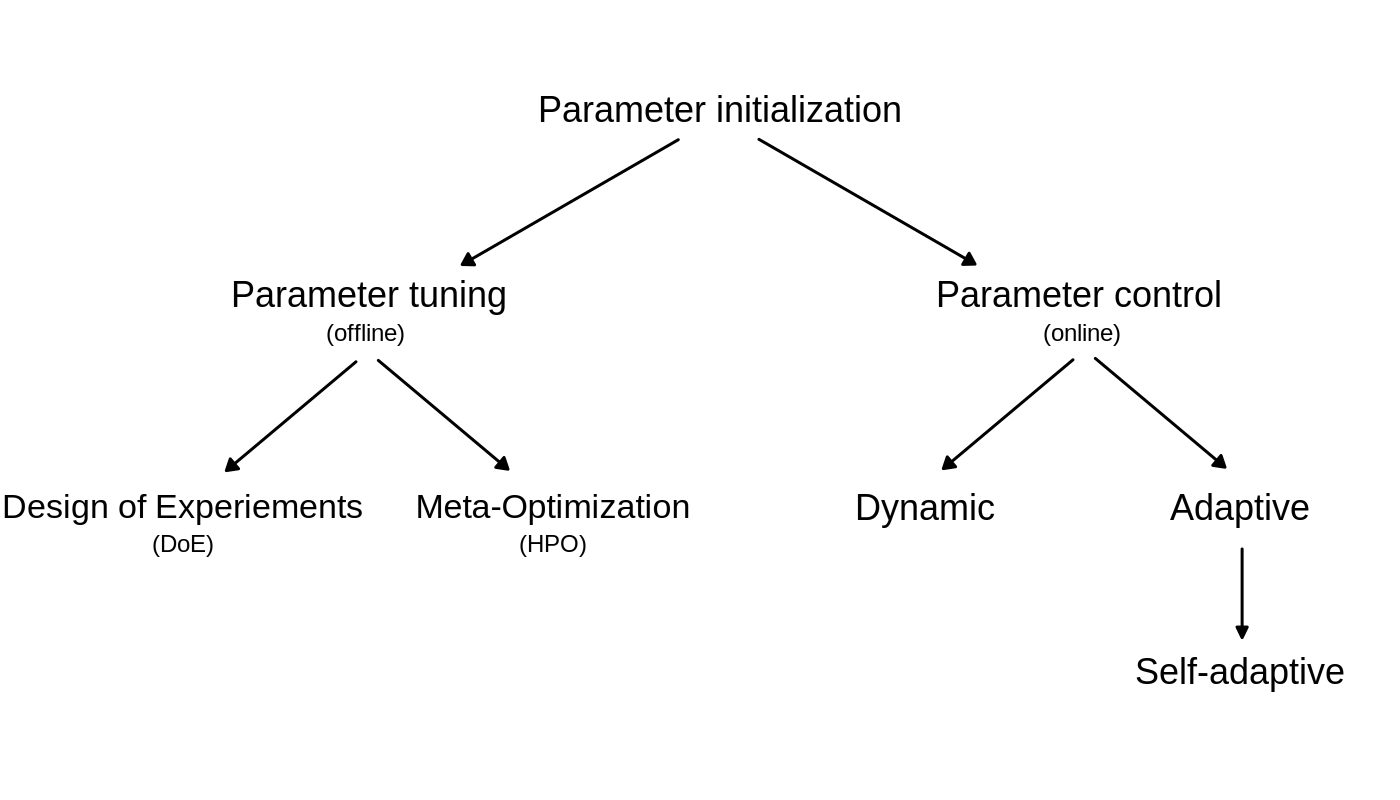
\includegraphics[width=0.9\textwidth]{metaheuristic_parameter_classification.svg}
	\caption[Taxonomy of parameter optimization]{Taxonomy of parameter optimization. Modified from \citet{eiben1999parameter}.}
	\label{fig:paramtax}
\end{figure}

This thesis applies methods from machine learning research to address this challenge. Therefore, the following review of parameter optimization methods classifies this technique and identifies other possible strategies. \Cref{fig:paramtax} shows a taxonomy of parameter optimization methods from \citet{eiben1999parameter}, with additions from \citet{talbi2009metaheuristics} and \citet{stutzle2012parameter}. There are two main differences: \enquote{Parameter Tuning} (offline initialization) tries to find good parameter settings before the algorithm is even applied, and these settings remain fixed afterwards. \enquote{Parameter Control} (online initialization) modifies the parameters while the algorithm is running, allowing for potentially better adaptation to the problem.

\subsubsection{Parameter Control}

Parameter control methods can be advantageous because they can adapt to the problem instance over time. They can also be used to encourage certain search phases of the algorithm, increasing either the exploratory or the exploitative behavior after a certain time. Several ways of implementing such online parameter initialization methods have been proposed. \textit{Deterministic} strategies alter the values according to a specific deterministic rule, while also allowing for minor random influences on the parameters. \textit{Adaptive} optimization, on the other hand, takes additional feedback from the metaheuristic algorithm to control the weight for its change, but still relies on predefined functions for this. Lastly, \textit{self-adaptive} parameter control implements the parameter change into the metaheuristic algorithm itself, making it part of its search space and thus the solution.

\subsubsection{Parameter Tuning}
\label{chap:tuning}

The simplest and oldest method of parameter tuning is a manual trial-and-error approach. By tuning one parameter at a time, each parameter is evaluated on its own, but without considering the interactions between them. This also becomes a very time consuming and error prone process as the parameter space grows.
Two methods address these issues with offline tuning. The first is a \gls{doe} approach to determine the minimum required scope of the experiments needed and to arrange the test points within the parameter space based on an optimality criterion. The result of these experiments should reveal a good set of parameters, with the possibility of further statistical significance tests.  
The other method uses meta-optimization, which is an algorithmic layer on top of the metaheuristic to find optimal parameter values. This can be either a metaheuristic algorithm (like \gls{pso}) or a machine learning based approach, which is discussed in the following subsection.


\subsection{Hyperparameter Optimization}
\label{chap:hyperopt}

In \gls{ml} applications hyperparameters are used to configure a \gls{ml} model. Similar to parameters in metaheuristics, tuned hyperparameters can greatly improve the performance of a \gls{ml} model over the default settings. In particular, state-of-the-art deep learning techniques, which have a large number of tunable parameters, can only be properly utilized if the hyperparameters are specifically tuned for their problem.

Traditionally, simple gradient descend-based approaches are often used for optimization problems. In its simplest form, the objective function $f(x)$ is to be minimized by $\min_{x \in \mathbb{R}} f(x)$, with a region of feasible values $D = \left\lbrace { x \in X | g_i(x) \leq 0, h_j(x) = 0}\right\rbrace $, and possible range and equality constraints $g_i(x), h_j(x)$ from a set of all values $X$. Following the negative gradient direction, a global optimum could be obtained for convex functions \cite{yang2020hyperparameter}. 
However, \gls{ml} models pose some challenges to these established techniques:
\begin{enumerate}
	\item The underlying objective function of a \gls{ml} model is usually not convex nor differentiable. Therefore, methods like gradient descend often result in local optima.
	\item The hyperparameters of \gls{ml} models are in the domain of continuous (real-valued),  discrete (integer-valued), binary, categorical and even conditional values. This results in a complex configuration space with sometimes non-obvious value ranges.
	\item Objective function evaluations can be very expensive, which necessitates methods for quicker, more efficient sampling. 
\end{enumerate}

In parallel with research on optimal parameters for metaheuristics (see \ref{chap:paramopt}), the manual tuning of hyperparameters in \gls{ml} applications began to become impractical in the face of more complex and feature-rich models. Therefore, interest in the automated tuning of hyperparameters, called \gls{hpo}, began in the 1990s. With important use cases being the reduction of human effort, the improved performance of these algorithms and, especially in scientific research, to help reproducibility, much progress has been made since the above-mentioned gradient descent-based methods were first applied  \cite{feurer2019hyperparameter}. 

The \gls{hpo} problem statement can be formulated as follows \cite{feurer2019hyperparameter}:
Let $\mathcal{A}$ be a \gls{ml} algorithm with $N$ hyperparameters, where $\Lambda_n$ denotes the $n$-th hyperparameter. The complete hyperparameter configuration space can then be defined as $\mathbf{\Lambda} = \Lambda_1 \times \Lambda_2 \times ... \times \Lambda_N$, with a vector of a possible hyperparameter configuration $\mathbf{\lambda} \in \mathbf{\Lambda}$. Thus, a \gls{ml} algorithm initialized with hyperparameters $\mathbf{\lambda}$ is denoted by $\mathcal{A}_\mathbf{\lambda}$.
Based on this, the process of \gls{hpo} consists of four main components: 1) an estimator (most often a regressor, but a classifier is also possible), 2) a search space $\mathbf{\Lambda}$, 3) a method to select configurations from the search space, and 4) a validation protocol $\mathcal{V}$ and its loss function $\mathcal{L}$ to evaluate the performance of the configuration (e.g., error rate or root mean squared error). 
The goal is then to find the optimal hyperparameter set $\mathbf{\lambda^*}$ on a given data set $\mathcal{D}$ divided into training data $D_\text{train}$ and validation data $D_\text{valid}$ that minimizes the error $\mathbb{E}$ from the validation protocol:
\begin{equation}
	\label{eq:hpo}
	\mathbf{\lambda^*} = \operatorname*{argmin}_{\mathbf{\lambda} \in \mathbf{\Lambda}} \mathbb{E}_{(D_\text{train}, D_\text{valid}) \sim \mathcal{D}} \left[ \mathcal{V}(\mathcal{L}, \mathcal{A}_\mathbf{\lambda}, D_\text{train}, D_\text{valid}) \right] 
\end{equation}

Almost all of this also applies to the parameter optimization for metaheuristic algorithms. Here, the loss function $\mathcal{L}$ is often closely related to the objective function itself, e.g., the resulting tour length in solutions to the \gls{tsp}. Therefore, \gls{hpo} for metaheuristics has no need for any supervised data sets or ground truths. Applied to metaheuristics solving the \gls{tsp}, with the solution quality function $f(\mathbf{s})$ from \cref{eq:solution_quality}, the \gls{hpo} goal from \cref{eq:hpo} can be defined as follows:
\begin{equation}
	\label{eq:hpo-meta}
	\mathbf{\lambda^*} = \operatorname*{argmin}_{\mathbf{\lambda} \in \mathbf{\Lambda}} \mathbb{E} \left[ \mathcal{V}(f, \mathcal{A}_\mathbf{\lambda}) \right] 
\end{equation}
with $\mathcal{A}_\mathbf{\lambda}$ now being the metaheuristic algorithm initialized with parameters $\mathbf{\lambda}$. To simplify all further explanations, let the objective function $f: \mathcal{\mathbf{\Lambda}} \to \mathbb{R}$ be defined directly by its parameter space $\mathcal{\mathbf{\Lambda}}$, which is mapped into the real solution quality space $\mathbb{R}$.

There are several ways to solve the above mentioned problem statements. A common distinction between these methods is their use of the objective function and its loss landscape. A \gls{hpo} algorithm can either treat this as a black-box function, using full evaluations of the objective function to model its behavior, or it can approach the problem with so-called \enquote{multi-fidelity optimization}, where the model is too complex and computationally expensive to use for evaluation and a cheap (possibly noisy) proxy is used instead \cite{feurer2019hyperparameter}. Another important distinction, especially in the area of black-box \gls{hpo}, is whether or not to use a statistical model, .i.e an estimator. Model-free techniques rely solely on function evaluation and factual improvement for their optimization process, without using any prior knowledge to sample the search space. Model-based methods, however, employ a more sophisticated strategy, often implemented using so-called \gls{bo}, which is explained in the next subsection. Other strategies for \gls{hpo} involve evolutionary algorithms or population-based methods, such as \gls{pso} \cite{yang2020hyperparameter}. Although, this approach of using metaheuristics to tune a metaheuristic is similar to the process proposed by \cite{talbi2009metaheuristics} (see \cref{chap:tuning}), it is not used in later stages of the thesis, due to its conflicting nature in the context of parameter optimization applied to a complex metaheuristic such as \gls{hsppbo}.

The following subsections give four examples of black-box \gls{hpo}, with one using model-free and the remaining using model-based, \gls{bo} techniques. All of these methods were also used for the experiments discussed in later sections of this thesis.

\subsection{Grid Search and Random Search}

A very simple and straightforward approach to \gls{hpo} is \gls{gs}. With its basic functionality similar to brute-force methods, it evaluates all possible combinations of hyperparameter values. \gls{gs} only requires finite sets of value ranges to be defined for each hyperparameter. It then iterates over the entire search space by creating the Cartesian product of these sets. This approach is easily interpretable and repeatable, while also being trivially implemented and parallelized \cite{bergstra2012random}. However, each new parameter causes the Cartesian product to grow exponentially, so \gls{gs} suffers greatly from the \enquote{curse of dimensionality}. Another problem is its inability to explore promising value ranges on its own. Since these must be predefined, a user would have to manually adjust these ranges before each run \cite{yang2020hyperparameter}.

\gls{rs} was proposed to overcome the limitations of \gls{gs} by sampling the hyperparameters from a probability distribution over the configuration space $F(\mathbf{\Lambda})$, eliminating the need to try all possible combinations \cite{bergstra2012random}. In most cases, this probability distribution is simply uniform for all hyperparameters, but certain applications may warrant for a higher density in some regions of a hyperparameter. \Cref{alg:randomsearch} presents the pseudo-code for the \gls{rs} algorithm. It basically compares each new function evaluation $f(\mathbf{\lambda_{\text{new}}})$ on a randomly sampled parameter $\mathbf{\lambda_{\text{new}}}$. The termination criterion is usually implemented as a fixed budget of function evaluations $B$, thus giving each of $N$ hyperparameters $B$ different evaluations, as opposed to $B^{1/N}$ with \gls{gs} (would it also operate on a fixed budget) \cite{bergstra2012random}. This gives parameters with a higher partial dependence on solution quality a much higher chance of finding a global optimum. It also shares the same advantages as \gls{gs}: easy implementation, parallelization and reproducibility (given a fixed random number generator). On the other hand, \gls{rs} (possibly) still evaluates unimportant search areas, since it has no guidance in its exploratory behavior, as a model-based \gls{hpo} algorithm might have \cite{yang2020hyperparameter}.
Nevertheless, it still serves as a well-performing baseline for many \gls{ml} benchmarks, with hyperparameters relatively close to the optimum, given sufficient resources \cite{feurer2019hyperparameter}.

\begin{algorithm}
	\caption{Random Search}
	\label{alg:randomsearch}
	\begin{algorithmic}
		\Require Probability distribution over parameter space $F(\mathbf{\Lambda})$
		\State Initialize parameters: $\mathbf{\lambda^*} \gets F(\mathbf{\Lambda})$
		\Repeat
		\State $\mathbf{\lambda_{\text{new}}} \gets F(\mathbf{\Lambda})$
		\If{$f(\mathbf{\lambda_{\text{new}}}) < f(\mathbf{\lambda^*}) $}
		\State $\mathbf{\lambda^*} \gets \mathbf{\lambda_{\text{new}}}$
		\EndIf
		\Until{termination criterion met}\\
		\Return $\mathbf{\lambda^*}$
	\end{algorithmic}
\end{algorithm}


\subsection{Bayesian Optimization}
\label{chap:bo}
\gls{bo} is not just an algorithm used for \gls{hpo}, but a complete framework for the global optimization of (expensive) black-box functions. It differs from methods like the aforementioned \gls{rs} by incorporating prior knowledge about the objective function into the sampling procedure. 
The prior, i.e., the analyzed objective function $f: \mathcal{\mathbf{\Lambda}} \to \mathbb{R}$, under the assumption of the evident data, it samples $\mathcal{D}_t = \left\lbrace (\mathbf{\lambda_i}, f(\mathbf{\lambda_i})) |  i\in [1,t] \right\rbrace $ yields a likelihood $P(\mathcal{D}_t|f)$, which can then be combined with the prior distribution $P(f)$ leading to the posterior distribution by applying Bayes' theorem:
\begin{equation}
	P(f|\mathcal{D}_t) \propto P(\mathcal{D}_t|f) P(f)
\end{equation}
In essence, this expresses the likelihood of the sampled data under the assumptions made for the objective function \cite{brochu2010tutorial}. 
Applying this in practice means that more sampled data points will cause the posterior function to adjust its mean for those points, reducing its uncertainties and increasing its predictive power \cite{williams2006gaussian}. 

 
\begin{algorithm}
	\caption{Bayesian Optimization}
	\label{alg:bo}
	
	\begin{algorithmic}
		\State Initialize parameters: $\mathbf{\lambda^*} \gets F(\mathbf{\Lambda})$
		\State $y_{min} = f(\mathbf{\lambda^*}) + \epsilon$
		\State \Call{InitializeModel}{$\mathcal{D}_\text{init}$}
		\For{$t \in [1,\text{n\_calls}]$}
		\State $\mathbf{\lambda_t} = \operatorname*{argmax}_{\mathbf{\lambda}} u(\mathbf{\lambda}|\mathcal{D}_{t-1})$ \Comment{acquisition function}
		\State $y_t = f(\mathbf{\lambda_t}) + \epsilon_t$
		\State $\mathcal{D}_t = \left\lbrace \mathcal{D}_{t-1}, (\mathbf{\lambda_t}, f_t) \right\rbrace $
		\State \Call{UpdateModel}{$\mathcal{D}_t$}
		\If{$y_t  < y_{min}$}
		\State $y_{min} = y_t$
		\State $\mathbf{\lambda^*} = \mathbf{\lambda_t}$
		\EndIf
		\EndFor
		\\
		\Return $\lambda^*$
	\end{algorithmic}
\end{algorithm}

A common interpretation of this theory for effective implementations of \gls{bo} is an iterative algorithm, given by \Cref{alg:bo}, consisting of two main parts: a surrogate model analogous to the posterior function over the objective and an acquisition function that guides the sampling process to the optimum. After initializing the model with an optional number of initial samples $\mathcal{D}_\text{init}$, a maximum of \textit{n\_calls} are made to the objective function $f$, with the following process for each iteration: 
First, the acquisition function $u(\mathbf{\lambda}|\mathcal{D}_{t-1})$ uses the probability distribution of the surrogate and all previously sampled data points to evaluate the search space to find the most beneficial next point to sample. High acquisition corresponds to potentially optimal objective function values. By selecting widely unsampled parameter areas, the function realizes exploratory behavior, while further sampling in already well-performing areas employs exploitative strategies. The specific choice of the acquisition function always defines a (customizable) trade-off between these two \cite{brochu2010tutorial}. 
With the most promising parameter input $\mathbf{\lambda_t}$ of iteration $t$ specified, the (potentially) noisy objective function $f(\mathbf{\lambda_t}) + \epsilon_t$ gets sampled. The noise is often modeled as an independent Gaussian distribution with zero mean and variance $\sigma_n^2$:
\begin{equation}
	\label{eq:gauss-noies}
	\epsilon = \mathcal{N}(0,\sigma_n^2)
\end{equation} 
following the original proposition of \citet{williams2006gaussian}.
Afterwards, the probabilistic surrogate model is fitted to the observations $\mathcal{D}_t$, which implements the update procedure of the algorithm. This surrogate model ideally represents the actual objective function as closely as possible, while also being mathematically advantageous and easy to compute \cite{feurer2019hyperparameter}. A standard choice for this would be a \gls{gp}, although many other models can be used, such as \gls{rf} or \gls{gbrt}.
An example of the process can be seen in \cref{fig:bo-sample}, which shows the first three iterations of \gls{bo} applied to a 1D toy function, using a \gls{gp} surrogate with two initial random samples.

\begin{figure}[h]
	\centering
	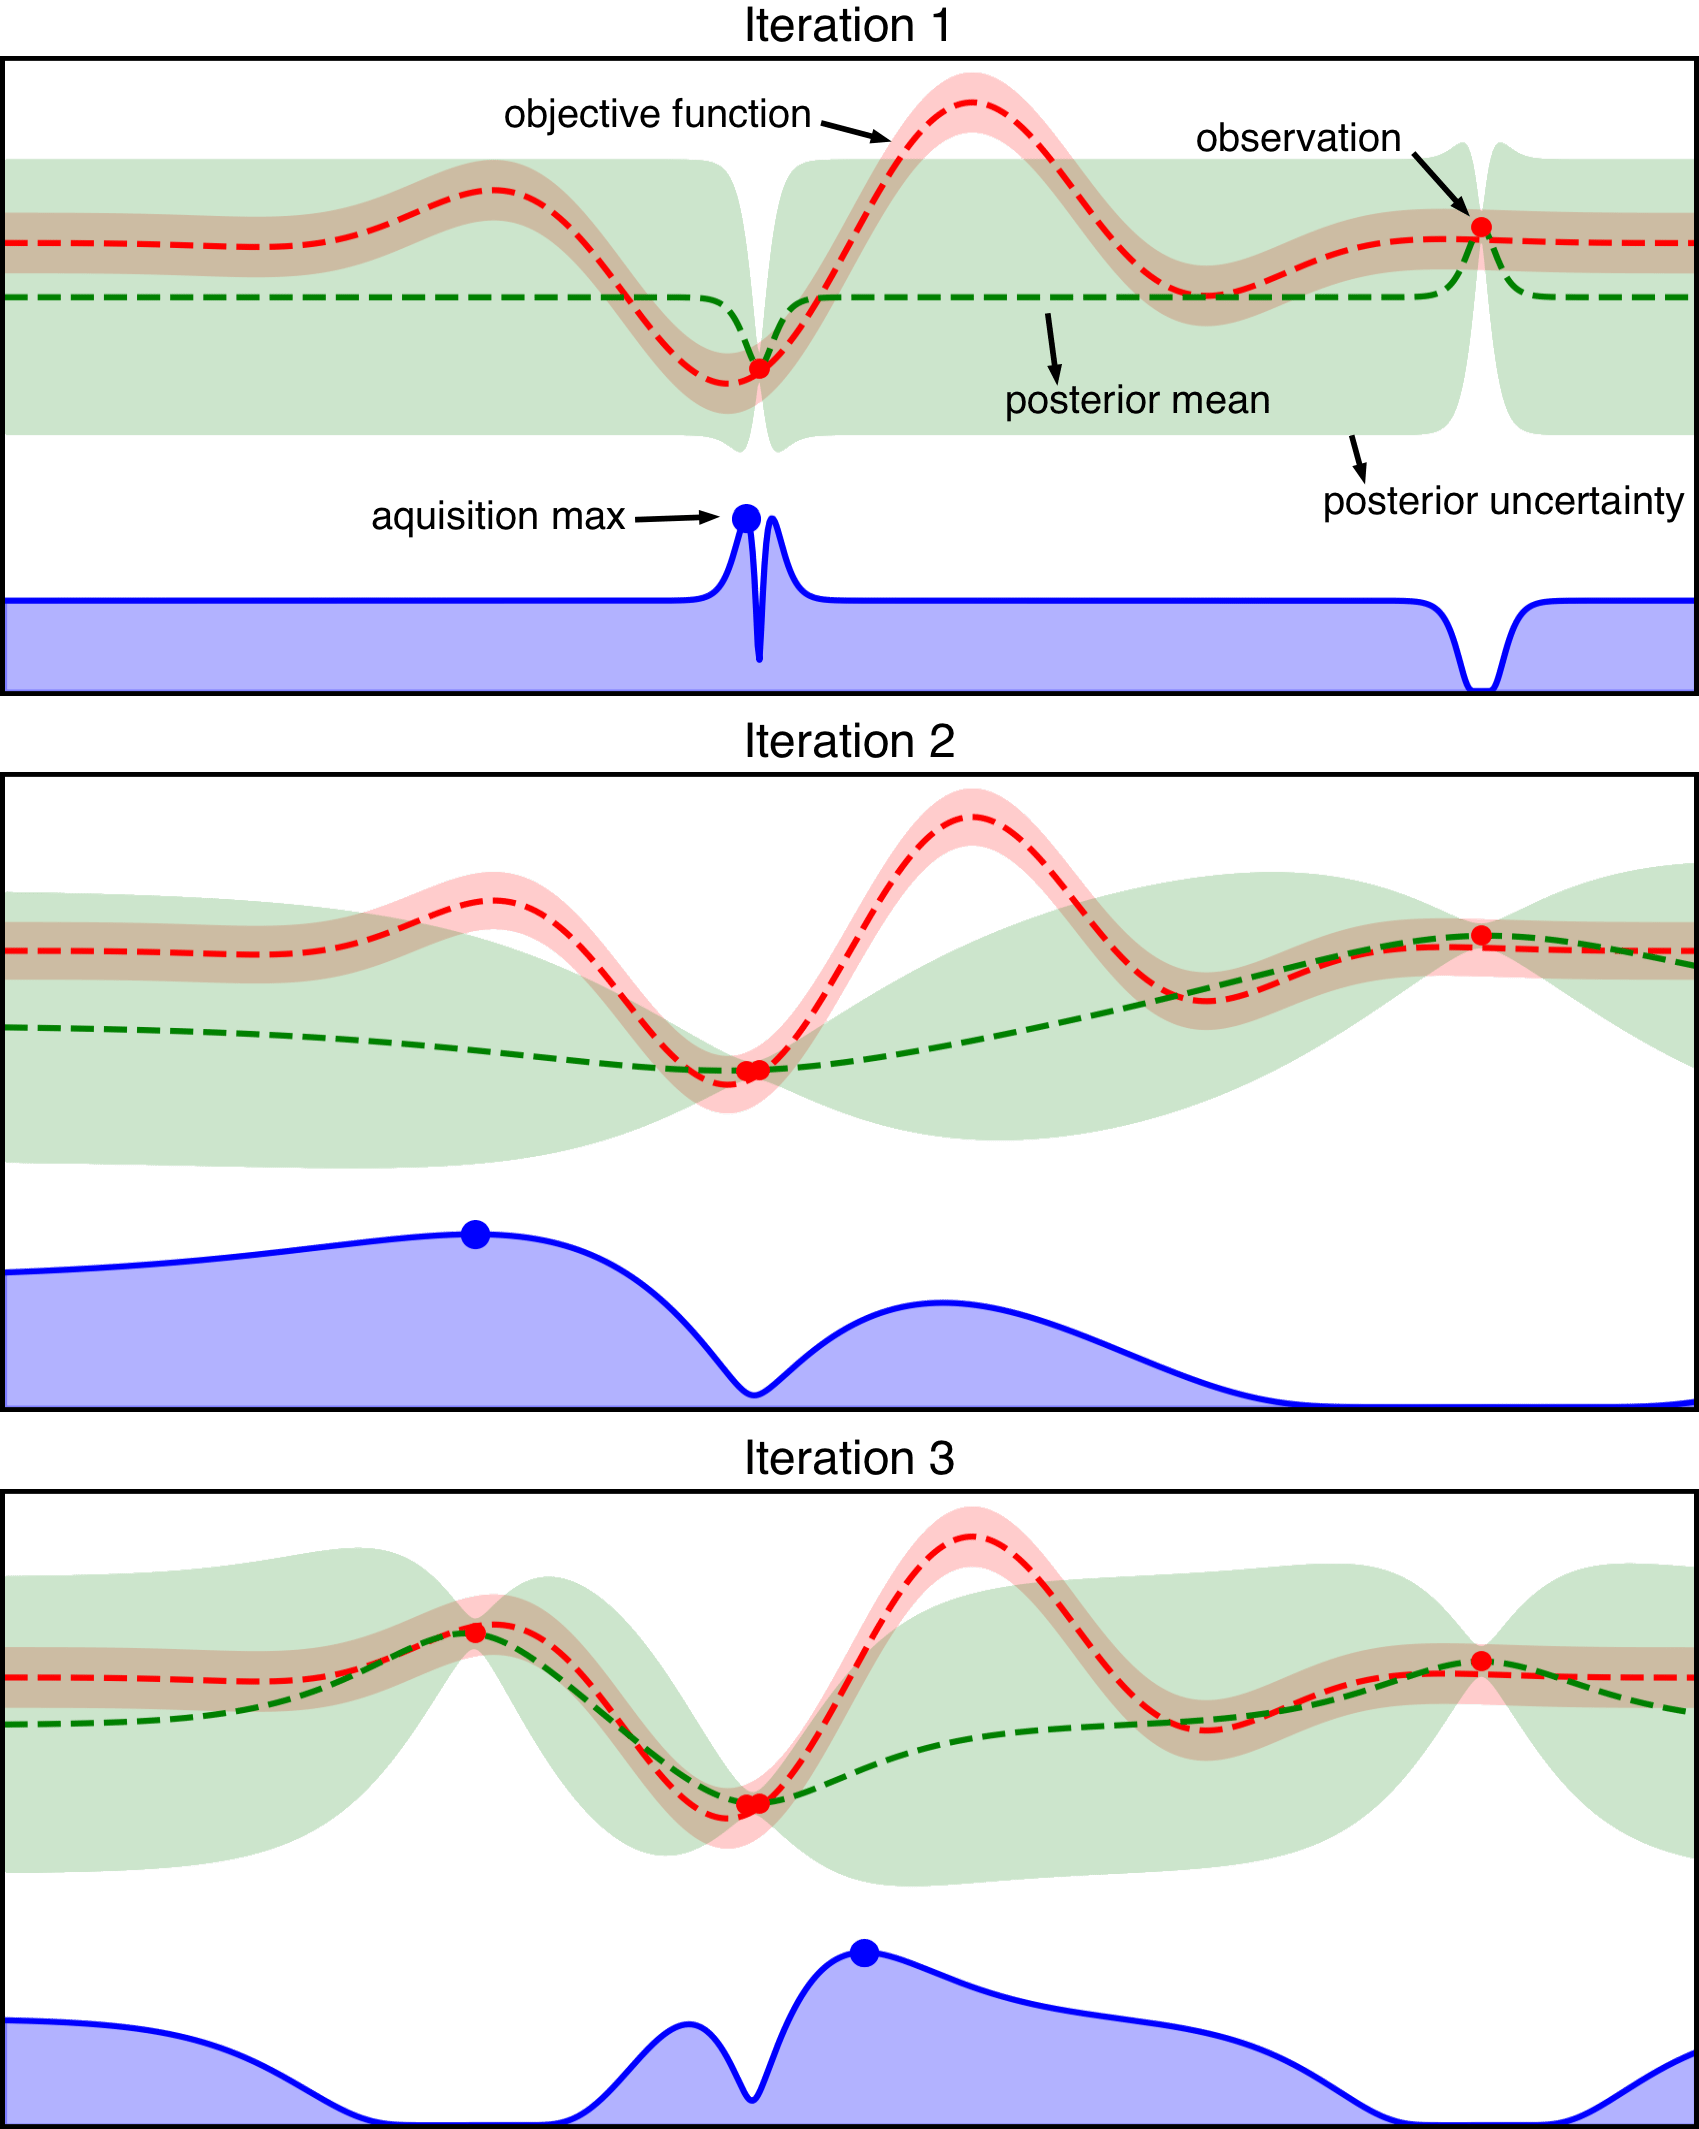
\includegraphics[width=0.7\textwidth]{bo-sample.png}
	\caption[An example of \gls{bo} using a \gls{gp} surrogate]{An example of \gls{bo} using a \gls{gp} surrogate (mean prediction as green dotted line, uncertainty as green tube) and an acquisition function (lower blue curve) on a noisy 1D toy function (red dotted line with red tube as noise).
		The figure shows three different iterations of the \gls{bo} process using two initial samples: The top shows the first iteration with only the samples to build the surrogate on and low acquisition values around these points. The middle shows the following iteration, including the newly sampled point, while reducing the uncertainty. The bottom shows that only after three iterations, almost half of the acquisition space has lost its value, and the surrogate model gains more accuracy around the samples.}
	\label{fig:bo-sample}
\end{figure}

Various combinations of surrogate model and acquisition function are possible in realizing a \gls{bo} algorithm. The relatively fast convergence to near-global optima makes this versatile algorithm a viable choice for \gls{hpo}, greatly improving on model-free methods. However, the sequential dependence on previously sampled data makes parallelization difficult \cite{yang2020hyperparameter}.
The following subsections briefly describe some popular acquisition functions and then discuss three surrogate models in more detail. These models were chosen based on their variance with respect to the \gls{bo} process. A more detailed justification is given in \cref{chap:opt-choice}.

\subsubsection{Acquisition Functions}
\label{chap:bo-acq}

As mentioned before, an acquisition function guides the sampling process, balancing exploration and exploitation. Given the distribution of the surrogate model, including its predictive mean $\mu(\mathbf{\lambda})$, its variance function $\sigma(\mathbf{\lambda})$, and the previously sampled data $\mathcal{D}$, where $f_{min} = \operatorname*{argmin}_{\mathbf{\lambda}\in \mathcal{D}} f(\mathbf{\lambda})$ is the best observed value so far, the acquisition function is defined as $u: \mathbf{\Lambda} \to \mathbb{R}^+$ \cite{snoek2012practical}. Two common choices for this function are the \gls{pi} and the \gls{ei}.

\paragraph{Probability of Improvement}
\gls{pi} as proposed by \citet{kushner1964new} attempts to maximize the probability of improving over the current best value $f_{min}$, with little regard for the comparative amount of improvement in less certain but more promising environments. With a trade-off parameter $\xi \geq 0$ to control this shortcoming, and $\Phi(\cdot)$ denoting the  \gls{cdf} of the standard normal, the resulting acquisition function is:
\begin{equation}
	\text{PI}(\mathbf{\lambda}) = P(f(\mathbf{\lambda}) < f_{min} + \xi)  
	= \Phi \left(  \frac{f_\text{min} - \mu(\mathbf{\lambda}) - \xi}{\sigma(\mathbf{\lambda})} \right) 
\end{equation}
This process is greedy by nature, but offers a guaranteed improvement of at least $\xi$ \cite{brochu2010tutorial}.

\paragraph{Expected Improvement}
As proposed by \citet{jones1998efficient}, \gls{ei} improves on \gls{pi} by also considering the magnitude of potential improvement a sample may yield. The goal is to calculate the expected deviation from a potential sample $f(\mathbf{\lambda})$ and the current minimum $f_\text{min}$, so
\begin{equation}
	\text{EI}(\mathbf{\lambda}) = \mathbb{E}[\max(f_\text{min}-f(\mathbf{\lambda}),0)].
\end{equation}
This allows the sample to be chosen to give a maximum improvement over the previous best observation.
\gls{ei} can also be expressed in a closed form with an additional trade-off parameter $\xi \geq 0$ to balance exploration and exploitation. Using the standard normal \gls{cdf} $\Phi(\cdot)$ and standard normal \gls{pdf} $\phi(\cdot)$, the equation is defined as follows:
\begin{equation}
	\label{eq:ei}
	\text{EI}(\mathbf{\lambda}) = (f_\text{min} - \mu(\mathbf{\lambda}) - \xi) \cdot \Phi(Z)+\sigma(\mathbf{\lambda})\cdot \phi(Z) 
\end{equation} 
$$
Z =  \frac{f_\text{min} - \mu(\mathbf{\lambda}) - \xi}{\sigma(\mathbf{\lambda})} 
$$
The first addend of \cref{eq:ei} realizes the exploitation of the function, favoring high means, while the second addend handles the exploration, selecting points with large surrogate variances \cite{brochu2010tutorial}.


\subsubsection{Surrogate Model: Gaussian Process}
A standard choice for a surrogate model is the \gls{gp}. As an extension of the multivariate Gaussian distribution, a \gls{gp} is defined by any finite number $N$ of variables (parameters) $\mathbf{\lambda}$, or in this case by their mean $m(\mathbf{\lambda})$, and a covariance function $k(\mathbf{\lambda},\mathbf{\lambda}^{\prime})$:
\begin{equation}
	f(\mathbf{\lambda}) \sim \mathcal{GP}(m(\mathbf{\lambda}), k(\mathbf{\lambda},\mathbf{\lambda}^{\prime}))
\end{equation}
with the mean function most often taken to be zero, so that the process solely relies on the covariance function, whose specification assumes a distribution over the objective function \cite{williams2006gaussian}. The default choice for this so-called \textit{kernel} (implying the use of the \textit{kernel trick}) in the original proposal is a squared exponential function, which specifies the covariance between pairs of random variables $\mathbf{\lambda_i},\mathbf{\lambda_j}$ as:
\begin{equation}
	k(\mathbf{\lambda_i},\mathbf{\lambda_j}) = \exp \left(  -\frac{1}{2} \lVert \mathbf{\lambda_i} - \mathbf{\lambda_j} \rVert^2 \right) 
\end{equation}

Then, using the Sherman-Morrison-Woodbury formula, a predictive distribution for the function value at the next iteration $t+1$ can be expressed by:
\begin{equation}
	P(f_{t+1} | \mathcal{D}_t, \mathbf{\lambda_{t+1}} ) = \mathcal{N}(\mu_t(\mathbf{\lambda_t+1}), \sigma^2_t(\mathbf{\lambda_t+1}))
\end{equation}
where $\mu$ and $\sigma^2$ denote the mean and variance of the model, and can be calculated using the kernel matrix over the covariance function (see \cite[p.8]{brochu2010tutorial}).
A disadvantage of the squared exponential kernel is that it assumes a very smooth objective function, which is unrealistic for real physical processes \cite{stein1999interpolation}.  
Instead, a Matérn kernel is often suggested as a replacement. It uses a parameter $\upsilon$ to control  smoothness, and common settings for \gls{ml} applications are $\upsilon = 3/2$ and $\upsilon=5/2$ \cite{williams2006gaussian}.

The default \gls{gp} scales cubically with the number of data points, which limits the number of function evaluations. Another issue is poor scalability to higher dimensions, which is attempted to be overcome by using other kernels \cite{feurer2019hyperparameter}.


\subsubsection{Surrogate Model: Random Forest}
\label{chap:rf}
Very different from \gls{gp} are the next two approaches, which come from the field of ensemble methods often used in \gls{ml}. The basic idea of these methods is to train several so-called \enquote{base learners} $h_1(\mathbf{\lambda}), ...,h_J(\mathbf{\lambda})$ (sometimes also referred to as \enquote{weak learners}), which are easy to fit and infer on, but have poor individual generalization performance due to very high variance. The base learners are then combined to produce a final predictor of the objective function $\hat{f}(\mathbf{\lambda}) (\approx f(\mathbf{\lambda}))$. In the case of regression, which applies to \gls{hpo}, this means a simple average of all base learners \cite{cutler2012random}:
\begin{equation}
	\label{eq:avg-est}
	\hat{f}(\mathbf{\lambda}) = \frac{1}{J} \sum_{j=1}^{J} h_j(\mathbf{\lambda})
\end{equation}

\gls{rf} is one of these methods, and was first introduced under this name by \citet{breiman2001random} as an improvement on his bagging algorithm for decision trees.
Each base learner, as described above, is a binary partitioned regression tree, where each partition or \enquote{split} is based on a predictor variable $\lambda_i \in \mathbf{\lambda}$ (i.e., the hyperparameters). A split may be done by value range for a continuous variable, or by choosing a subset $S$ from the set of all categories $S_i$ for categorical variables (see \Cref{fig:decision-tree}). A splitting criterion is used to evaluate all possible splits among all variables, and then the most descriptive split is chosen. For regression, the mean squared error is often used for this task, while classification typically uses the Gini index to calculate the \enquote{purity} of each potential class \cite{cutler2012random}. 

\begin{figure}
	\centering
	\resizebox{0.9\textwidth}{!}{
		\begin{forest} decision tree
			[$\lambda_i < a$,plain content
			[left descendant;{yes},plain content,elo={yshift=2pt}]
			[right descendant;{no},plain content,elo={yshift=2pt}]
			]
		\end{forest}
		\quad
		\begin{forest} decision tree
			[$\lambda_i \in S \subset S_i$,plain content
			[left descendant;{yes},plain content,elo={yshift=2pt}]
			[right descendant;{no},plain content,elo={yshift=2pt}]
			]
	\end{forest}}
	\caption[Example of decision trees]{Example of two decision trees. (Left) Splitting a continuous variable $\lambda_i$ at point $a$. (Right) Splitting a categorical variable $\lambda_i$ via subset $S$.}
	\label{fig:decision-tree}
\end{figure}

The bagging algorithm now improves on the foundation of decision trees \cite{breiman1996bagging}. Given a data set $\mathcal{D}$ of size $n$, consisting of pairs of $N$ parameters $\mathbf{\lambda} = \left\lbrace \lambda_1,...,\lambda_N\right\rbrace $ and their corresponding function value $y = f(\mathbf{\lambda})$, bagging repeatedly selects a random subset of the same size $n$ as the original data set, but with replacement, thus allowing for duplicates and possible unused values or \enquote{out-of-bag} data. This process is called \enquote{bootstrap sampling} and reduces overfitting, while also allowing the out-of-bag data to be used to validate the estimator. The tree is then fitted using this sample as described above.
\gls{rf} introduces more randomization into the decision tree building process by taking not only a subset of the available data for each base learner, but also taking a random sample (with replacement) of size $m$, where $m < N$ of the predictor values for each split. As a result, the base learners do not overfit to presumably highly predictive variables, which reduces the correlation among the sub-sampled data sets and increases the accuracy of the ensemble prediction \cite{ho2002data}. The resulting implementation template is described in \cref{alg:random-forest}. The process can also be easily parallelized since each base learner is constructed individually \cite{cutler2012random}.

\begin{algorithm}
	\caption{Random Forests}
	\label{alg:random-forest}
	\begin{algorithmic}
		\For{$j=1$ to $J$}
			\State $\mathcal{D}_j \subseteq \mathcal{D}$ \Comment{sample with replacement, $|\mathcal{D}_j| = |\mathcal{D}|$}
			\Procedure{CreateTree}{$\mathcal{D}_j, m$} $ \to h_j(\mathbf{\lambda})$
				\State Start with all observations in root node
				\ForAll{unsplit nodes, recursivley}
					\State Randomly select $m$ predictor variables
					\State Split the node according to the best binary split among these $m$ variables
				\EndFor
			\EndProcedure
		\EndFor
		\Return $\hat{f}(\mathbf{\lambda})$ \Comment{using \cref{eq:avg-est}}
	\end{algorithmic}
\end{algorithm}

\paragraph{Extremely Randomized Trees}
As the name suggests, the extremely randomized trees approach proposed by \citet{geurts2006extremely} introduces another step of randomization into the process. While the main part of this algorithm, often called \gls{et}, is based on random forests, the split points for each node of the decision tree are now chosen completely randomly, as opposed to being based on the best split among all available predictor variables. To explain further, the sampled $m$ predictor variables are each randomly split once, evaluated (e.g., using the mean squared error) and then the best performing split is chosen for the current node. In addition, each base learner is now built using the entire data set, rather than just a bootstrap sample. The motivation behind \gls{et} is to reduce variance through random splits and minimize bias by using the full data set, while also having the potential to improve the computational time needed to build the estimator.

\subsubsection{Surrogate Model: Gradient Boosted Trees}

\gls{gbrt} is also an ensemble method that uses decision trees as base learners to produce an ensemble prediction, and was originally proposed by \citet{friedman2001greedy}. However, unlike \gls{rf}, which averages many full-depth decision trees, \gls{gbrt} sequentially builds many small, high-bias decision trees (depth $d \approx 4$), improving on each other using the residuals from the last iteration. The schematic architecture of this approach is outlined in \cref{fig:gbrt}.
\begin{figure}
	\centering
	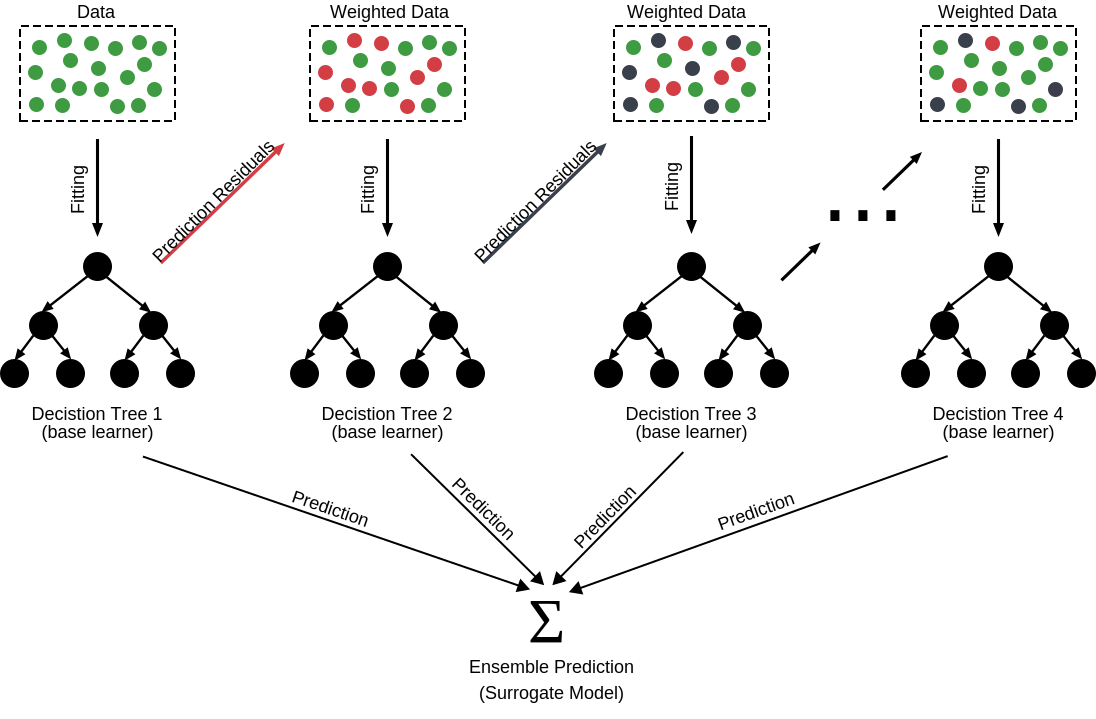
\includegraphics[width=\textwidth]{gbrt.svg}
	\caption[Schematic view of \gls{gbrt}]{Schematic view of \gls{gbrt}. Modified from \citet{deng2021ensemble}.}
	\label{fig:gbrt}
\end{figure}
For simplicity, let $f_j = f_j(\mathbf{\lambda})$. The ensemble regressor $\hat{f}_j$ is the $j$-th of all $J$ estimators in an additive sequence 
\begin{equation}
	\label{eq:add-gbrt}
	\hat{f}_j = \hat{f}_{j-1} + \upsilon \cdot h_j
\end{equation}
where $\upsilon \in (0,1]$ is a \enquote{shrinkage} parameter that controls the learning rate, leading to better generalization \cite{friedman2002stochastic}.
Let $\mathcal{L}(f,\hat{f})$ be the loss function for the estimator. Now, at each iteration $j$, a new base learner $h_j$ is added to the ensemble by minimizing over its sum of losses for the entire data set $\mathcal{D}$ ($|\mathcal{D}| = n$), with $(\mathbf{\lambda}_i, y_i)$ being the $i$-th element of $\mathcal{D}$\footnote{Note that this is an exception to the previously established notation of $\mathbf{\lambda}_i$ being the $i$-th parameter in the configuration.} and $y_i = f(\mathbf{\lambda}_i)$ \cite{friedman2001greedy}:
\begin{equation}
	\label{eq:gbrt-tree}
	h_j = \operatorname*{argmin}_{h} \sum_{i=1}^{n} \mathcal{L}(y_i, \hat{f}_{j-1}(\mathbf{\lambda}_i) + h(\mathbf{\lambda}_i))
\end{equation}
To make this a computationally closed-form, a first-order Taylor approximation to the loss-function is used to obtain the following term:
\begin{equation}
	\mathcal{L}(y_i, \hat{f}_{j-1}(\mathbf{\lambda}_i) + h(\mathbf{\lambda}_i)) \approx \mathcal{L}(y_i, \hat{f}_{j-1}(\mathbf{\lambda}_i)) + h_j(\mathbf{\lambda}_i) \left[ \frac{\partial\mathcal{L}(y_i, \hat{f}(\mathbf{\lambda}_i))}{\partial \hat{f}(\mathbf{\lambda}_i)} \right]_{\hat{f}=\hat{f}_{j-1}}
\end{equation}
The derivative of this equation can be understood as the gradient $g_{ij}$ of the loss function, where a steepest descent following $-g_{ij}$ is desired. To summarize, in each of the $J$ iterations, a decision tree of fixed depth $d$ is fitted using all predictor variables to minimize the negative gradient of the all $n$ data points:
\begin{equation}
	h_j \approx -\operatorname*{argmin}_{h} \sum_{i=1}^{n} (h(\mathbf{\lambda}_i) - g_{ij})^2
\end{equation}
Given a typical squared error loss function $\mathcal{L}(f, \hat{f}) = \frac{1}{2}(f - \hat{f})^2$, the negative gradient can be simplified to an ordinary residual $r_{ij} = -g_{ij} = y_i - \hat{f}_{j-1}(\mathbf{\lambda}_i)$ \cite[Chapter~10]{hastie2009elements}.

Lastly, \cref{alg:gbrt} describes the high-level implementation of \gls{gbrt} using a squared loss function and a decision tree building process, as described with \gls{rf} in \cref{chap:rf}, using a continuous update for the residuals ($r_{i} \gets r_{ij}$, for current iteration $j$) \cite{mohan2011web}.
Although this algorithm uses a constant initialization for the residuals, other methods could be used as well.

\begin{algorithm}
	\caption{Gradient Boosted Regression Trees (Squared Loss)}
	\label{alg:gbrt}
	\begin{algorithmic}
		\State Initialization: $\forall i \in [1,n]: r_i = y_i$
		\For{$j=1$ to $J$}
			\State$h_j \gets$ \Call{CreateTree}{$\left\lbrace (\mathbf{\lambda_1}, r_1), ..., (\mathbf{\lambda_n}, r_n)\right\rbrace$, $d$}
			\For{$i=1$ to $n$}
				\State $r_i \gets r_i - \upsilon \cdot h_j(\mathbf{\lambda_i})$
			\EndFor
		\EndFor
		\State $\hat{f} = \upsilon \cdot \sum_{j=1}^{J} h_j$
		\State \Return $\hat{f}$
	\end{algorithmic}
\end{algorithm}


\subsection{Example: Bayesian Optimization for the H-SPPBO}
To better understand how the \glsdesc{hpo} process works with a metaheuristic such as the \gls{hsppbo}, the following is a theoretical example using the mathematical symbols and formula from above. This example focuses on \gls{bo} using a \gls{rf} surrogate model, and the underlying problem to be solved is the \gls{tsp}.

Let the \gls{hsppbo} algorithm, as explained in \cref{chap:hsppbo}, be denoted by $\mathcal{A}_\mathbf{\lambda}$ with its parameters initialized by the parameter vector $\mathbf{\lambda}$. This parameter vector is an element of the parameter configuration space $\mathbf{\Lambda} = \Lambda_1 \times \Lambda_2 \times ... \times \Lambda_N = w_{\text{persprev}} \times w_{\text{persbest}} \times w_{\text{parentbest}} \times \alpha \times \beta \times \theta \times H \times L$. Furthermore, let each solution constructed by $\mathcal{A}_\mathbf{\lambda}$ be defined as a vector $\mathbf{s} = (s_1,...,s_n) \in V^n$, where $V$ is the set containing all possible city nodes of the \gls{tsp} problem description. Assuming, that random influences can be ignored, the function describing this solution construction depends only on the parameters and is denoted as $g(\mathbf{\lambda}) = \mathbf{s}$. The quality of each solution $f : V^n \rightarrow \mathbb{R}_{0}^{+}$ is then defined as the tour length $L$ given by the weights/distances between each of the nodes, described by \cref{eq:solution_quality}, so $f(\mathbf{s}) = L$. Since these solutions are depend only on the parameters $\mathbf{\lambda}$ with which the \gls{hsppbo} algorithm $\mathcal{A}_\mathbf{\lambda}$ was initialized, again assuming no random influences, the function definition  $\mathbf{\lambda} \to_{g} V^n \to_{f} \mathbb{R}_{0}^{+}$ can be simplified to directly output the length $L$ for any given parameter vector $\mathbf{\lambda}$. Thus, the only function necessary for the metaheuristic is now defined as $f(\mathbf{\lambda}) = L = y$, where $y$ is used to conform to the previous notation for \gls{hpo}.

Now, given the \glsdesc{hpo} goal from \cref{eq:hpo-meta}, we have defined the solution quality function $f$ and the algorithm $\mathcal{A}_\mathbf{\lambda}$, as well as a configuration space $\mathbf{\Lambda} $. In addition, let $F(\mathbf{\Lambda})$ denote a sampling function that chooses a parameter set $\mathbf{\lambda}$ under a uniform distribution, let $u: \mathbf{\Lambda} \to \mathbb{R}^+$ be an arbitrary acquisition function, and let $\mathcal{D}_t = \left\lbrace (\mathbf{\lambda_i}, y_i) |  i\in [1,t] \right\rbrace $ be the data set consisting of the parameter pairs and their corresponding solution qualities, sampled so far during the \gls{hpo} process.

Starting with the \gls{bo} process, we first obtain an initial data set $\mathcal{D}_\text{init}$ using our sampling function $F(\mathbf{\Lambda})$. For example, the first entry of this set might contain, among the other parameters, the two values $\alpha = 8, \beta = 2$, resulting in a solution quality (tour length) of $y = 100$, and a second entry might contain the values $\alpha = 7, \beta = 3$, resulting in a solution quality of $y=90$, so $\left\lbrace ((...,8,2,...), 100), ((...,7,3,...), 90) \right\rbrace \subset \mathcal{D}_\text{init}$. Based on this data, the first \gls{rf} model is built as explained in \cref{chap:rf}. For example, the first base learner $h_j(\mathbf{\lambda})$ built in the ensemble of all $J$ learners could select $\alpha < 7.5$ as a split node for the decision tree with a predicted solution quality of $y=100$ for the side where the condition is true, and $y=90$ otherwise. This split was chosen because following the prediction of this decision tree using the parameters from the data set $\mathcal{D}_\text{init}$ resulted in the lowest mean squared error of all possible splits. Note, that this explanation is an oversimplification of the actual process. 

From this split, all further child nodes are also split until some termination criterion is met, e.g. the mean squared error is below a certain threshold. Now that we have trained our base learners, we average over their predictions, resulting in our predictor $\hat{f}(\mathbf{\lambda}) = \hat{y}$. This predictor, or surrogate model in terms of the \gls{bo}, is ideally as close as possible to the actual objective function $f(\mathbf{\lambda}) = y$ that we defined earlier. However, the predictor only learns a relationship between an input parameter set and the resulting solution quality (tour length $L$), not the actual solution path $\mathbf{s}$. Ignoring possible \gls{ml}-related effects such as overfitting, the more parameter pairs and corresponding solution qualities we have, the more accurate our predictor will be. Nevertheless, since we do not want to run hundreds or thousands of expensive real objective function calls, we use the \gls{bo} process, to acquire only new data points that maximize our benefit for training this predictor - quality over quantity of data.

As we progress in the \gls{bo} process, we can use our trained surrogate model for the acquisition function $u(\cdot)$ to determine the most beneficial new point in the parameter configuration space $\mathbf{\Lambda}$. To do this, we need to compute the mean and variance over our surrogate model and its parameter inputs (see \cref{chap:bo-acq}). The resulting new point from $u$, which is a parameter set $\mathbf{\lambda}$, is evaluated by the real objective function, the \gls{hsppbo}, and this new data point $(\mathbf{\lambda}, y)$ is added to $\mathcal{D}_t$ in the $t$-th iteration of the \gls{bo} algorithm (see \cref{alg:bo}). The \gls{rf} surrogate model is then trained again, but now with this new data point, which should increase its accuracy. This process is repeated until a certain number of predetermined objective calls \texttt{n\_calls} have been evaluated. Finally, the \gls{bo} algorithm returns the parameter set $\mathbf{\lambda}^*$ from the iteration that produced the best solution quality $y$. We also get the final trained surrogate model $\hat{f}(\mathbf{\lambda})$.